\section{Squark and Gluino Production at Tree Level}\label{sec:SquarkGluinoTree}
This chapter considers the production of strongly interacting supersymmetric particles in the MRSSM\footnote{In fact only the RSQCD is considered as contribution coming from the electroweak sector scale with $\alpha_w = \frac{g_w^2}{4\pi}$ or $\alpha_{\mathrm{em}} = \frac{e^2}{4\pi}$ and are therefore significantly smaller than contribution from the strongly interacting sector which scale with $\alpha_s = \frac{g_s^2}{4\pi}$.} The various processes and their associated cross section are compared to their analogues in the MSSM.\\
The production of sgluons is not included in the following analysis. However, there are two possible channels for sgluon production at tree-level: a quark-antiquark and a gluon-gluon initiated process:
\begin{align}
q\overline{q} \to \phi_0\phi_0\ (\sigma_0\sigma_0), \hspace{2cm} GG \to \phi_0\phi_0\ (\sigma_0\sigma_0).
\end{align}
To give a reasonable and consistent prediction of hadronic cross sections, a scenario with large sgluon mass, i.e. soft breaking parameter $m_\sigma = \unit[5]{TeV}$, is considered. This validates the negligence of sgluon production as in this case they are too heavy to significantly produce them at the LHC with $\sqrt{S} = \unit[13]{TeV}$. See \cite{Choi:2008ub, GoncalvesNetto:2012nt, phdWojciech} for a calculation of the sgluon production cross section. \ignore{Feynman diagrams there are only ones, one can only produce sigma,sigma or phi,phi but not sigma,phi}
Section \ref{sec:PartProcesses} gives analytic results for the parton reaction before the next section describes how the hadronic cross section is obtained. Section \ref{sec:tree-level_cross_sections} presents the hadronic cross section of all considered processes for various choices of squark and gluino mass. In particular, squark production is considered more closely. This includes the statement of uncertainties of the calculation.




\subsection{Partonic Processes and their Cross Section}\label{sec:PartProcesses}
\begin{figure}[!htbp]
\begin{center}
\begin{tikzpicture}[line width=1.0 pt, scale=1.3, arrow/.style={thick,->,shorten >=2pt,shorten <=2pt,>=stealth}]
	\draw[fermion] (-1,0.5)--(-0.42,0);
	\draw[fermionbar] (-1,-0.5)--(-0.42,0);
	\draw[gluon] (-0.42,0)--(0.42,0); 
	\draw[scalar] (0.42,0)--(1,0.5);
	\draw[scalarbar] (0.42,0)--(1,-0.5);
	\draw[arrow] (-1,0.7)--(-0.5,0.26);
	\node at (-0.75,0.8) {$k_a$};
	\draw[arrow] (-1,-0.7)--(-0.5,-0.26);
	\node at (-0.75,-0.8) {$k_b$};
	\draw[arrow] (0.5,0.26)--(1,0.7);
	\node at (0.75,0.8) {$p_1$};
	\draw[arrow] (0.5,-0.26)--(1,-0.7);
	\node at (0.75,-0.8) {$p_2$};
\begin{scope}[shift={(3,0)}]
	\draw[fermion] (-1,0.5)--(0,0.5);
	\draw[fermionbar] (-1,-0.5)--(0,-0.5);
	\draw[fermionnoarrow] (0,0.5)--(0,-0.5);
	\draw[gluon] (0,0.5)--(0,-0.5); 
	\draw[scalar] (0,0.5)--(1,0.5);
	\draw[scalarbar] (0,-0.5)--(1,-0.5);
\end{scope}
\end{tikzpicture}
%\caption{Tree level diagrams for $q\overline{q} \to \tilde{q}\tilde{q}^\dagger$}
\end{center}
%\end{figure}
%\begin{figure}[!htbp]
\begin{center}
\begin{tikzpicture}[line width=1.0 pt, scale=1.3]
    \node at (0,0) {};
\begin{scope}[shift={(0,-1)}]
	\draw[gluon] (-1,0.5)--(-0.42,0);
	\draw[gluon] (-1,-0.5)--(-0.42,0);
	\draw[gluon] (-0.42,0)--(0.42,0); 
	\draw[scalar] (0.42,0)--(1,0.5);
	\draw[scalarbar] (0.42,0)--(1,-0.5);
\begin{scope}[shift={(3,0)}]
	\draw[gluon] (-1,0.5)--(0,0.5);
	\draw[gluon] (-1,-0.5)--(0,-0.5);
	\draw[scalarbar] (0,0.5)--(0,-0.5);
	\draw[scalar] (0,0.5)--(1,0.5);
	\draw[scalarbar] (0,-0.5)--(1,-0.5);
\end{scope}
\begin{scope}[shift={(6,0)}]
	\draw[gluon] (-1,0.5)--(0,0.5);
	\draw[gluon] (-1,-0.5)--(0,-0.5);
	\draw[scalar] (0,0.5)--(0,-0.5);
	\draw[scalarnoarrow] (0,0.5)--(0.4,0.1);
	\draw[scalarbar] (0.6,-0.1)--(1,-0.5);
	\draw[scalarnoarrow] (0,-0.5)--(0.5,0);
	\draw[scalar] (0.5,0)--(1,0.5);
\end{scope}
\begin{scope}[shift={(9,0)}]
	\draw[gluon] (-1,0.5)--(0,0);
	\draw[gluon] (-1,-0.5)--(0,0);
	\draw[scalarbar] (0,0)--(1,-0.5);
	\draw[scalar] (0,0)--(1,0.5);
\end{scope}
\end{scope}
\end{tikzpicture}
%\caption{Tree level diagrams for $GG \to \tilde{q}\tilde{q}^\dagger$}
\end{center}
%\end{figure}
%\begin{figure}[!htbp]
\begin{center}
\begin{tikzpicture}[line width=1.0 pt, scale=1.3]
    \node at (0,0) {};
\begin{scope}[shift={(0,-1)}]
	\draw[fermion] (-1,0.5)--(0,0.5);
	\draw[fermion] (-1,-0.5)--(0,-0.5);
	\draw[gluon] (0,0.5)--(0,-0.5);
	\draw[fermionnoarrow] (0,0.5)--(0,-0.5);
	\draw[scalar] (0,0.5)--(1,0.5);
	\draw[scalar] (0,-0.5)--(1,-0.5);;
\begin{scope}[shift={(3,0)}]
	\draw[fermion] (-1,0.5)--(0,0.5);
	\draw[fermion] (-1,-0.5)--(0,-0.5);
	\draw[gluon] (0,0.5)--(0,-0.5);
	\draw[fermionnoarrow] (0,0.5)--(0,-0.5);
	\draw[scalarnoarrow] (0,0.5)--(0.4,0.1);
	\draw[scalar] (0.6,-0.1)--(1,-0.5);
	\draw[scalarnoarrow] (0,-0.5)--(0.5,0);
	\draw[scalar] (0.5,0)--(1,0.5);
\end{scope}
\end{scope}
\end{tikzpicture}
%\caption{Tree level diagrams for $qq \to \tilde{q}\tilde{q}$}
\end{center}
%\end{figure}
%\begin{figure}[!htbp]
\begin{center}
\begin{tikzpicture}[line width=1.0 pt, scale=1.3]
    \node at (0,0) {};
\begin{scope}[shift={(0,-1)}]
	\draw[fermion] (-1,0.5)--(-0.42,0);
	\draw[fermionbar] (-1,-0.5)--(-0.42,0);
	\draw[gluon] (-0.42,0)--(0.42,0); 
	\draw[gluon] (0.42,0)--(1,0.5);
	\draw[fermionnoarrow] (0.42,0)--(1,0.5);
	\draw[gluon] (0.42,0)--(1,-0.5);
	\draw[fermionnoarrow] (0.42,0)--(1,-0.5);
\begin{scope}[shift={(3,0)}]
	\draw[fermion] (-1,0.5)--(0,0.5);
	\draw[fermionbar] (-1,-0.5)--(0,-0.5);
	\draw[scalar] (0,0.5)--(0,-0.5);
	\draw[gluon] (0,0.5)--(1,0.5);
	\draw[fermionnoarrow] (0,0.5)--(1,0.5);
	\draw[gluon] (0,-0.5)--(1,-0.5);
	\draw[fermionnoarrow] (0,-0.5)--(1,-0.5);
\end{scope}
\begin{scope}[shift={(6,0)}]
	\draw[fermion] (-1,0.5)--(0,0.5);
	\draw[fermionbar] (-1,-0.5)--(0,-0.5);
	\draw[scalar] (0,0.5)--(0,-0.5);
	\draw[gluon] (0,0.5)--(0.4,0.1);
	\draw[fermionnoarrow] (0,0.5)--(0.4,0.1);
	\draw[gluon] (0.6,-0.1)--(1,-0.5);
	\draw[fermionnoarrow] (0.6,-0.1)--(1,-0.5);
	\draw[gluon] (0,-0.5)--(1,0.5);
	\draw[fermionnoarrow] (0,-0.5)--(1,0.5);
\end{scope}
\end{scope}
\end{tikzpicture}
%\caption{Tree level diagrams for $q\overline{q} \to \tilde{g}\overline{\tilde{g}}$}
\end{center}
%\end{figure}
%\begin{figure}[!htbp]
\begin{center}
\begin{tikzpicture}[line width=1.0 pt, scale=1.3]
    \node at (0,0) {};
\begin{scope}[shift={(0,-1)}]
	\draw[gluon] (-1,0.5)--(-0.42,0);
	\draw[gluon] (-1,-0.5)--(-0.42,0);
	\draw[gluon] (-0.42,0)--(0.42,0); 
	\draw[gluon] (0.42,0)--(1,0.5);
	\draw[fermionnoarrow] (0.42,0)--(1,0.5);
	\draw[gluon] (0.42,0)--(1,-0.5);
	\draw[fermionnoarrow] (0.42,0)--(1,-0.5);
\begin{scope}[shift={(3,0)}]
	\draw[gluon] (-1,0.5)--(0,0.5);
	\draw[gluon] (-1,-0.5)--(0,-0.5);
	\draw[gluon] (0,0.5)--(0,-0.5);	
	\draw[fermionnoarrow] (0,0.5)--(0,-0.5);
	\draw[gluon] (0,0.5)--(1,0.5);
	\draw[fermionnoarrow] (0,0.5)--(1,0.5);
	\draw[gluon] (0,-0.5)--(1,-0.5);
	\draw[fermionnoarrow] (0,-0.5)--(1,-0.5);
\end{scope}
\begin{scope}[shift={(6,0)}]
	\draw[gluon] (-1,0.5)--(0,0.5);
	\draw[gluon] (-1,-0.5)--(0,-0.5);
	\draw[gluon] (0,0.5)--(0,-0.5);
	\draw[fermionnoarrow] (0,0.5)--(0,-0.5);
	\draw[gluon] (0,0.5)--(0.4,0.1);
	\draw[fermionnoarrow] (0,0.5)--(0.4,0.1);
	\draw[gluon] (0.6,-0.1)--(1,-0.5);
	\draw[fermionnoarrow] (0.6,-0.1)--(1,-0.5);
	\draw[gluon] (0,-0.5)--(1,0.5);
	\draw[fermionnoarrow] (0,-0.5)--(1,0.5);
\end{scope}
\end{scope}
\end{tikzpicture}
%\caption{Tree level diagrams for $GG \to \tilde{g}\overline{\tilde{g}}$}
\end{center}
%\end{figure}
%\begin{figure}[!htbp]
\begin{center}
\begin{tikzpicture}[line width=1.0 pt, scale=1.3]
    \node at (0,0) {};
\begin{scope}[shift={(0,-1)}]
	\draw[fermion] (-1,0.5)--(-0.42,0);
	\draw[gluon] (-1,-0.5)--(-0.42,0);
	\draw[fermion] (-0.42,0)--(0.42,0); 
	\draw[scalar] (0.42,0)--(1,0.5);
	\draw[gluon] (0.42,0)--(1,-0.5);
	\draw[fermionnoarrow] (0.42,0)--(1,-0.5);
\begin{scope}[shift={(3,0)}]
	\draw[fermion] (-1,0.5)--(0,0.5);
	\draw[gluon] (-1,-0.5)--(0,-0.5);
	\draw[gluon] (0,0.5)--(0,-0.5);	
	\draw[fermionnoarrow] (0,0.5)--(0,-0.5);
	\draw[scalar] (0,0.5)--(1,0.5);
	\draw[gluon] (0,-0.5)--(1,-0.5);
	\draw[fermionnoarrow] (0,-0.5)--(1,-0.5);
\end{scope}
\begin{scope}[shift={(6,0)}]
	\draw[fermion] (-1,0.5)--(0,0.5);
	\draw[gluon] (-1,-0.5)--(0,-0.5);
	\draw[scalar] (0,0.5)--(0,-0.5);
	\draw[gluon] (0,0.5)--(0.4,0.1);
	\draw[fermionnoarrow] (0,0.5)--(0.4,0.1);
	\draw[gluon] (0.6,-0.1)--(1,-0.5);
	\draw[fermionnoarrow] (0.6,-0.1)--(1,-0.5);
	\draw[gluon] (0.6,-0.1)--(1,-0.5);
	\draw[fermionnoarrow] (0.6,-0.1)--(1,-0.5);
	\draw[scalarnoarrow] (0,-0.5)--(0.5,0);
	\draw[scalar] (0.5,0)--(1,0.5);
\end{scope}
\end{scope}
\end{tikzpicture}
\caption{Tree level diagrams for squark and gluino production at tree level in the MRSSM. The processes $GG \to \tilde{q}\overline{\tilde{q}}$ and $qG \to \tilde{q}\tilde{g}$ are identical to those in the MSSM. The processes $q\overline{q} \to \tilde{q}\overline{\tilde{q}}$ and $qq \to \tilde{q}\tilde{q}$ involve the production of less chiralities than in the MSSM. Also in the $q\tilde{q} \to \tilde{g}\overline{\tilde{g}}$ channel only half of the t-channel squark chiralities occur in the MRSSM. (Anti-)Gluino production via initial gluons $GG \to \tilde{g}\overline{\tilde{g}}$ proceeds via the same diagrams like in the MSSM but its cross section is twice as much in the MRSSM for gluino and antigluino are distinguishable particles.}\label{fig:TreeDiagrams}
\end{center}
\end{figure}
For the following calculation the top quark is excluded from the initial state as it is too heavy to be significantly present in protons. %Therefore its pdf is approximately zero. 
For consistency reasons also the stop is excluded from the final states. One therefore deals with $n_f-1 = 5$ quark flavors. In view of the renormalization and mass factorization to be performed at the 1-loop level, the results are calculated in (conventional) dimensional regularization (see section \ref{sec:RegSchemes}) and are therefore given in $D = 4 - 2\epsilon$ dimensions. Furthermore it has been distinguished between the gauge coupling $g_s$ from the gluon-quark-quark vertex and its supersymmetric analogue $\hat{g}_s$ from the gluino-squark-quark vertex. So far, it has not been distinguished between them because supersymmetry dictates them to be identical. However, the loop corrections to their corresponding vertex differ in dimensional regularization by a finite amount, as will be shown in section \ref{sec:renMRSSM}. To rectify this, an additional finite (supersymmetry restoring) counterterm needs to be added to one of renormalization constants of $g_s$ or $\hat{g}_s$. This will be done in \ref{sec:SUSYrestore}.\\
To parametrize results, the usual Mandelstam variables $s,t,u$ and the following modifications of them are used\footnote{The kinematics of the process is denoted in fig. \ref{fig:TreeDiagrams}.}
\begin{align}
& s = (k_a + k_b)^2 = (p_1 + p_2)^2,\nonumber\\
& t = (k_a - p_1)^2 = (k_b - p_2)^2,\nonumber\\
& u = (k_a - p_2)^2 = (k_a - p_2)^2,\nonumber\\
& t_{\tilde{g}} = t - m_{\tilde{g}}^2, && t_{\tilde{q}} = t- m_{\tilde{q}}^2,\nonumber\\
& u_{\tilde{g}} = u - m_{\tilde{g}}^2, && u_{\tilde{q}} = u- m_{\tilde{q}}^2.
\end{align}
Applying the Feynman rules in the Appendix \ref{sec:FeynmanRules}, one obtains the following sums\footnote{The sum $\sum$ denotes the summation over all external spins and colors.} over absolute squared Feynman amplitudes:
\begin{align}
\sum|\mathcal{M}^B|^2(q_i\overline{q}_j \to \tilde{q}\tilde{q}^\dagger) &= \delta_{ij}  \left[ 8 N_c C(F) g_s^4\frac{(n_f-1)}{s^2} + 4 N_c C(F) \hat{g}_s^4\frac{1}{t_{\tilde{g}}^2} - 8 C(F)g_s^2\hat{g}_s^2\frac{1}{ t_{\tilde{g}} s} \right] (tu-m_{\tilde{q}}^4)\nonumber\\
 &+ (1-\delta_{ij}) 4 N_c C(F) \hat{g}_s^4\frac{tu-m_{\tilde{q}}^4}{t_{\tilde{g}}^2}, \\
\sum|\mathcal{M}^B|^2(GG \to \tilde{q}\tilde{q}^\dagger) &= 4 (n_f-1) g_s^4 \left[ 2N_c^2C(F) \left(1 - 2\frac{t_{\tilde{q}}u_{\tilde{q}}}{s^2} \right)- 2C(F) \right]\nonumber\\
& \left[ 1 - \epsilon - 2\frac{s m_{\tilde{q}}^2}{t_{\tilde{q}}u_{\tilde{q}}} \left( 1-\frac{s m_{\tilde{q}}^2}{t_{\tilde{q}}u_{\tilde{q}}} \right)\right],\\
\sum|\mathcal{M}^B|^2(q_i q_j \to \tilde{q}\tilde{q}) &= \delta_{ij} 2\hat{g}_s^4 N_c C(F)\left[ \frac{1}{t_{\tilde{g}}^2} + \frac{1}{u_{\tilde{g}}^2} \right] (tu-m_{\tilde{q}}^4)\nonumber\\ 
& + (1-\delta_{ij}) 4 \hat{g}_s^4 N_c C(F) \frac{tu-m_{\tilde{q}}^4}{t_{\tilde{g}}^2},\\
\sum|\mathcal{M}^B|^2(q\overline{q} \to \tilde{g}\overline{\tilde{g}}) &=  8 N_c^2 C(F) g_s^4 \left[ \frac{2m_{\tilde{g}}^2 s + t_{\tilde{g}}^2 + u_{\tilde{g}}^2}{s^2} -\epsilon \right]\nonumber\\
& + 4 N_c^2 C(F) g_s^2 \hat{g}_s^2 \left[ \frac{m_{\tilde{g}}^2 s + t_{\tilde{g}}^2}{s t_{\tilde{q}}} + \frac{m_{\tilde{g}}^2 s + u_{\tilde{g}}^2}{su_{\tilde{q}}} + \epsilon\left( \frac{t_{\tilde{g}}}{t_{\tilde{q}}} + \frac{u_{\tilde{g}}}{u_{\tilde{q}}} \right) \right]\nonumber\\
& + 2C(F)(N_c^2-1) \hat{g}^4_s \left( \frac{t_{\tilde{g}}^2}{t_{\tilde{q}}^2} + \frac{u_{\tilde{g}}^2}{u_{\tilde{q}}^2} \right)\\
%& + 2 \hat{g}_s^4\left[ 2 N_c^2 C(F) \left( \frac{t_{\tilde{g}}^2}{t_{\tilde{q}}^2} + \frac{u_{\tilde{g}}^2}{u_{\tilde{q}}^2} \right) + 2 C(F) \left( 2\frac{m_{\tilde{g}}^2 s}{t_{\tilde{q}}u_{\tilde{q}}} - \frac{t_{\tilde{g}}^2}{t_{\tilde{q}}^2} - \frac{u_{\tilde{g}}^2}{u_{\tilde{q}}^2} \right) \right],\\
\sum|\mathcal{M}^B|^2(GG \to \tilde{g}\overline{\tilde{g}}) &=  16 N_c^3 C(F) g_s^4 \left( 1- \frac{t_{\tilde{g}}u_{\tilde{g}}}{s^2} \right)\nonumber\\
&\left[ \frac{s^2}{t_{\tilde{g}}u_{\tilde{g}}}(1-\epsilon)^2-2(1-\epsilon) + 4\frac{m_{\tilde{g}}^2 s}{t_{\tilde{g}}u_{\tilde{g}}}\left(1-\frac{m_{\tilde{g}}^2 s}{t_{\tilde{g}}u_{\tilde{g}}}  \right) \right],\\
\sum|\mathcal{M}^B|^2(qG \to \tilde{q}\tilde{g}) &=  2g_s^2\hat{g}_s^2 \left[ 2 N_c^2 C(F) \left(1-2\frac{s u_{\tilde{q}}}{t_{\tilde{g}}^2}\right) - 2C(F) \right] \nonumber\\
&\left[ (-1+\epsilon)\frac{t_{\tilde{g}}}{s} + \frac{2(m_{\tilde{g}}^2-m_{\tilde{q}}^2)t_{\tilde{g}}}{s u_{\tilde{q}}}\left( 1+\frac{m_{\tilde{q}}^2}{u_{\tilde{q}}} + \frac{m_{\tilde{g}}^2}{t_{\tilde{g}}} \right) \right].
\end{align}
The absolute squared amplitudes have been checked with the mathematica output generated by the packages  \texttt{FeynArts} \cite{Hahn:2000} and \texttt{FormCalc} \cite{ChokoufeNejad:2013qja, Hahn:1998yk} which used a model file for the MRSSM generated by \texttt{SARAH}\cite{Staub:2013tta, Staub:2012pb, Staub:2010jh, Staub:2009bi}.\\ 
Having calculated the absolute squared Feynman amplitudes one obtains the partonic cross sections (see Appendix \ref{sec:cross_section}) via
\begin{align}
\frac{\mbox{d}^2 \sigma^B}{\mbox{d}t\ \mbox{d}u} =& \frac{K_{ab}}{s^2} \frac{\pi S_{\epsilon}}{\Gamma(1-\epsilon)} \left[ \frac{tu-m_1^2m_2^2}{\mu^2 s}\right]^{-\epsilon} \Theta(tu-m_1^2m_2^2)\nonumber\\
&\ \Theta(s-4m^2) \delta(s+t+u-m_1^2-m_2^2) \sum |\mathcal{M}^B|^2,\label{eq:sigma_tree}
\end{align}
where $m_1$ ($m_2$) is the mass of the first (second) final state particle and $m$ is their arithmetic mean. The leading order cross sections then evaluate to
\begin{align}
\sigma^B(q_i \overline{q}_j \to \tilde{q}\tilde{q}^\dagger) &= \delta_{ij}  \frac{g_s^4}{16\pi s} (n_f-1) \left[ \frac{4}{27} - \frac{16 m_{\tilde{q}}^2}{27s} \right]\nonumber\\
&+ \delta_{ij} \frac{g_s^2\hat{g}_s^2}{16\pi s}  \left[ \left( \frac{4}{27} + \frac{8 m_-^2}{27 s} \right)\beta_{\tilde{q}}  + \left( \frac{8m_{\tilde{g}}^2}{27s} + \frac{8m_-^4}{27s^2} \right)L_1 \right]\nonumber\\
& + \frac{\hat{g}_s^4}{16\pi s} \left[ -\frac{8}{9}\beta_{\tilde{q}} + \left( -\frac{4}{9} - \frac{8m_-^2}{9s} \right)L_1 \right],\\
\sigma^B(GG \to \tilde{q}\tilde{q}^\dagger) &= \frac{(n_f-1) g_s^4}{16\pi s} \left[ \left(\frac{5}{24} + \frac{31 m_{\tilde{q}}^2}{12s}\right)\beta_{\tilde{q}} + \left( \frac{4m_{\tilde{q}}^2}{3s} + \frac{m_{\tilde{q}}^4}{3s^2} \right) \ln \frac{1-\beta_{\tilde{q}}}{1+\beta_{\tilde{q}}} \right],\\
\sigma^B(q_i q_j \to \tilde{q}\tilde{q}) &= \frac{\hat{g}_s^4}{16\pi s} \left[ -\frac{8}{9}\beta_{\tilde{q}} +  \left( -\frac{4}{9} - \frac{8m_-^2}{9s} \right)L_1 \right],\\
\sigma^B(q \overline{q} \to \tilde{g}\overline{\tilde{g}}) &= \frac{g_s^4}{16\pi s} \left[ \frac{16}{9} + \frac{32m_{\tilde{g}}^2}{9s} \right] \beta_{\tilde{g}}\nonumber\\
& + \frac{\hat{g}_s^2 g_s^2}{16\pi s}  \left[ \left( -\frac{4}{3}-\frac{8m_-^2}{3s} \right)\beta_{\tilde{g}} + \left( \frac{8 m_{\tilde{g}}^2}{3s} + \frac{8m_-^4}{3s^2} \right) L_2 \right]\nonumber\\
& + \frac{\hat{g}_s^4}{16\pi s} \left[ \left( \frac{32}{27} + \frac{32 m_-^4}{27(m_-^4 + m_{\tilde{q}}^2s)} \right)\beta_{\tilde{g}} - \frac{64m_-^2}{27s}L_2 \right],\label{eq:qqbar_to_sgsgbar}\\
\sigma^B(GG \to \tilde{g}\overline{\tilde{g}}) &= \frac{g_s^4}{16\pi s} \left[ \left( -6 - \frac{51 m_{\tilde{g}}^2}{2s} \right)\beta_{\tilde{g}} + \left( -\frac{9}{2} - \frac{18 m_{\tilde{g}}^2}{s} + \frac{18 m_{\tilde{g}}^4}{s^2} \right)\ln \frac{1-\beta_{\tilde{g}}}{1+\beta_{\tilde{g}}} \right],\\
\sigma^B(q G \to \tilde{q} \tilde{g}) &= \frac{g_s^2\hat{g}_s^2}{16\pi s} \left[ \frac{\kappa}{s}\left( -\frac{7}{9} - \frac{32 m_{-}^2}{9s} \right) + \left( -\frac{8m_-^2}{9s} + \frac{2m_{\tilde{q}}^2m_-^2}{s^2} + \frac{8 m_-^4}{9s^2} \right)L_3\right.\nonumber\\
&+\left. \left( -1-\frac{2m_-^2}{s} + \frac{2m_{\tilde{q}}m_-^2}{s^2} \right)L_4 \right],
\end{align}
where the abbreviations \cite{Beenakker:1996ch} 
\begin{align}
&\beta_{\tilde{q}} = \sqrt{1-\frac{4 m_{\tilde{q}}^2}{s}} && \beta_{\tilde{g}} = \sqrt{1-\frac{4 m_{\tilde{g}}^2}{s}}\nonumber\\
&m_-^2 = m_{\tilde{g}}^2 - m_{\tilde{q}}^2 && \kappa = \sqrt{(s-m_{\tilde{g}}^2-m_{\tilde{q}}^2)^2-4m_{\tilde{g}}^2m_{\tilde{q}}^2}\nonumber\\
& L_1 = \ln \frac{s+2m_-^2 - s\beta_{\tilde{q}}}{s+2m_-^2 + s\beta_{\tilde{q}}} && L_2= \ln \frac{s - 2m_-^2 - s\beta_{\tilde{g}}}{s - 2m_-^2 + s\beta_{\tilde{g}}}\nonumber\\
& L_3 = \ln \frac{s - m_-^2 - \kappa}{s - m_-^2 + \kappa} && L_4= \ln \frac{s + m_-^2 - \kappa}{s + m_-^2 + \kappa}
\end{align}
have been used. In the following, the considered processes of the MRSSM are compared to those of the MSSM.

\subsubsection*{The process $q_i \overline{q}_j \to \tilde{q}\tilde{q}^\dagger$}
The production of a squark and an antisquark through a quark and an antiquark in the initial state originates from two types of Feynman diagrams. The first one has an $s$-channel gluon and is the same in the MSSM and in the MRSSM. The second one exhibits a difference due to the $t$-channel gluino which is no Majorana particle in the MRSSM. 
\begin{figure}[!htbp]
\begin{center}
\begin{tikzpicture}[line width=1.0 pt, scale=1.3]
	\draw[fermion] (-1,0.5)--(-0.42,0);
	\draw[fermionbar] (-1,-0.5)--(-0.42,0);
	\draw[gluon] (-0.42,0)--(0.42,0); 
	\draw[scalar] (0.42,0)--(1,0.5);
	\draw[scalarbar] (0.42,0)--(1,-0.5);
\begin{scope}[shift={(3,0)}]
	\draw[fermion] (-1,0.5)--(0,0.5);
	\draw[fermionbar] (-1,-0.5)--(0,-0.5);
	\draw[fermionnoarrow] (0,0.5)--(0,-0.5);
	\draw[gluon] (0,0.5)--(0,-0.5); 
	\draw[scalar] (0,0.5)--(1,0.5);
	\draw[scalarbar] (0,-0.5)--(1,-0.5);
\end{scope}
\end{tikzpicture}
\caption{Tree level diagrams for $q\overline{q} \to \tilde{q}\tilde{q}^\dagger$}
\end{center}
\end{figure}
To see this one can either just apply the Feynman rules in Appendix \ref{sec:FeynmanRules} or think of the conservation of $R$-charge: Left handed squarks have R-charge $+1$ and right handed squarks have $R$-charge $-$1. Antiparticles have the opposite $R$-charge of their corresponding particles. The final state particles have to meet the total $R$-charge zero from the initial state. Because of this, one only has $\tilde{q}_L \overline{\tilde{q}}_L$ and $\tilde{q}_R \overline{\tilde{q}}_R$ as the final states in the MRSSM whereas in the MSSM one actually has four instead of two t-channel diagrams: The corresponding final states are $\tilde{q}_L \overline{\tilde{q}}_L$, $\tilde{q}_R \overline{\tilde{q}}_R$, $\tilde{q}_L \overline{\tilde{q}}_R$ and $\overline{\tilde{q}}_R \tilde{q}_L$. Consequently contributions from the $t$-channel diagrams are suppressed in the MRSSM in comparison to the MSSM. As visible in fig. \ref{fig:TreeXsection} this suppression grows with the masses. The reason for this lies in the gluino mass dependence of the $t$-channel diagrams which is explained in the discussion of squark production.\\
If the initial state quarks are of different flavor, the $s$-channel diagram is absent.

\subsubsection*{The process $GG \to \tilde{q}\tilde{q}^\dagger$}
This process has the same cross section as in the MSSM for also in the MSSM only like chirality squark and antisquark $\tilde{q}_A\tilde{q}_A^\dagger$ with $A \in \left\{L,R\right\}$ can be produced. 

\subsubsection*{The process $q_i q_j \to \tilde{q}\tilde{q}$}
In the MRSSM only the production of unlike chirality squarks $\tilde{q}_L \tilde{q}_R$ is allowed whilst in the MSSM also like chirality squarks can be produced. This is again a consequence of the conservation of R-charge. The upshot of this is a suppression of squark production in the MRSSM in comparison to the MSSM. To be more explicit the suppression of squark production in the MRSSM grows with the gluino mass. This can be understood as follows: As in the MRSSM a left handed squark needs to be produced with a right handed squark one can read off, from the Feynman rules given in Appendix \ref{sec:FeynmanRules}, that the gluino propagator $i\frac{\slashed{p}+m_{\tilde{g}}}{p^2-m_{\tilde{g}}^2}$ is sandwiched between the projectors $P_L$ and $P_R$ which leads to the cancellation of the gluino mass in the numerator. Therefore for small momenta of the gluino compared to the gluino mass one gets $\mathcal{M}$ $\sim m_{\tilde{g}}^{-2}$ in the MRSSM while in the MSSM one finds a suppression proportional to $m_{\tilde{g}}^{-1}$.\\
When considering squark production, one has to sum over all $|\mathcal{M}|^2$ with different helicity. The diagrams for those different final state helicities are shown for flavor like squark production in tab. \ref{tab:squark_likeflavor} and for flavor unlike squark production in tab. \ref{tab:squark_unlikeflavor} for the MSSM and the MRSSM. To avoid double counting one needs to weight $|\mathcal{M}|^2(qq\to \tilde{q}_L\tilde{q}_L)$ and $|\mathcal{M}|^2(qq\to \tilde{q}_R\tilde{q}_R)$ with a statistical factor of $\frac{1}{2}$ as one integrates over the momenta of both particles in $t$- and $u$-channel diagram to arrive at the cross section.
\begin{table}[!htpb]
\begin{center}
\begin{tabular}{c|c}
MSSM & MRSSM \\
\hline
\begin{tikzpicture}[line width=1.0 pt, scale=0.7]
	\draw[fermion] (0,1)--(1,1);
	\draw[fermion] (0,0)--(1,0);
	\draw[fermionnoarrow] (1,1)--(1,0);
	\draw[gluon] (1,1)--(1,0);
	\draw[scalar] (1,1)--(2,1);
	\draw[scalar] (1,0)--(2,0);
	\node at (-0.2,1) {$u$};
	\node at (-0.2,0) {$u$};
	\node at (2.5,1) {$\tilde{u}_L^\dagger$};
	\node at (2.5,0) {$\tilde{u}_R^\dagger$};
\begin{scope}[shift={(4,0)}]
	\draw[fermion] (0,1)--(1,1);
	\draw[fermion] (0,0)--(1,0);
	\draw[fermionnoarrow] (1,1)--(1,0);
	\draw[gluon] (1,1)--(1,0);
	\draw[scalar] (1,1)--(1.5,0.5);
	\draw[scalar] (1.5,0.5)--(2,0);
	\draw[scalar] (1,0)--(1.4,0.4);
	\draw[scalar] (1.6,0.6)--(2,1);
	\node at (-0.2,1) {$u$};
	\node at (-0.2,0) {$u$};
	\node at (2.5,1) {$\tilde{u}_L^\dagger$};
	\node at (2.5,0) {$\tilde{u}_R^\dagger$};
\end{scope}
\begin{scope}[shift={(0,-2)}]
	\draw[fermion] (0,1)--(1,1);
	\draw[fermion] (0,0)--(1,0);
	\draw[fermionnoarrow] (1,1)--(1,0);
	\draw[gluon] (1,1)--(1,0);
	\draw[scalar] (1,1)--(2,1);
	\draw[scalar] (1,0)--(2,0);
	\node at (-0.2,1) {$u$};
	\node at (-0.2,0) {$u$};
	\node at (2.5,1) {$\tilde{u}_L^\dagger$};
	\node at (2.5,0) {$\tilde{u}_L^\dagger$};
\end{scope}
\begin{scope}[shift={(4,-2)}]
	\draw[fermion] (0,1)--(1,1);
	\draw[fermion] (0,0)--(1,0);
	\draw[fermionnoarrow] (1,1)--(1,0);
	\draw[gluon] (1,1)--(1,0);
	\draw[scalar] (1,1)--(1.5,0.5);
	\draw[scalar] (1.5,0.5)--(2,0);
	\draw[scalar] (1,0)--(1.4,0.4);
	\draw[scalar] (1.6,0.6)--(2,1);
	\node at (-0.2,1) {$u$};
	\node at (-0.2,0) {$u$};
	\node at (2.5,1) {$\tilde{u}_L^\dagger$};
	\node at (2.5,0) {$\tilde{u}_L^\dagger$};
\end{scope}
\begin{scope}[shift={(0,-4)}]
	\draw[fermion] (0,1)--(1,1);
	\draw[fermion] (0,0)--(1,0);
	\draw[fermionnoarrow] (1,1)--(1,0);
	\draw[gluon] (1,1)--(1,0);
	\draw[scalar] (1,1)--(2,1);
	\draw[scalar] (1,0)--(2,0);
	\node at (-0.2,1) {$u$};
	\node at (-0.2,0) {$u$};
	\node at (2.5,1) {$\tilde{u}_R^\dagger$};
	\node at (2.5,0) {$\tilde{u}_R^\dagger$};
\end{scope}
\begin{scope}[shift={(4,-4)}]
	\draw[fermion] (0,1)--(1,1);
	\draw[fermion] (0,0)--(1,0);
	\draw[fermionnoarrow] (1,1)--(1,0);
	\draw[gluon] (1,1)--(1,0);
	\draw[scalar] (1,1)--(1.5,0.5);
	\draw[scalar] (1.5,0.5)--(2,0);
	\draw[scalar] (1,0)--(1.4,0.4);
	\draw[scalar] (1.6,0.6)--(2,1);
	\node at (-0.2,1) {$u$};
	\node at (-0.2,0) {$u$};
	\node at (2.5,1) {$\tilde{u}_R^\dagger$};
	\node at (2.5,0) {$\tilde{u}_R^\dagger$};
\end{scope}
\end{tikzpicture} & \begin{tikzpicture}[line width=1.0 pt, scale=0.7]
	\draw[fermion] (0,1)--(1,1);
	\draw[fermion] (0,0)--(1,0);
	\draw[fermionnoarrow] (1,1)--(1,0);
	\draw[gluon] (1,1)--(1,0);
	\draw[scalar] (1,1)--(2,1);
	\draw[scalar] (1,0)--(2,0);
	\node at (-0.2,1) {$u$};
	\node at (-0.2,0) {$u$};
	\node at (2.5,1) {$\tilde{u}_L^\dagger$};
	\node at (2.5,0) {$\tilde{u}_R^\dagger$};
\begin{scope}[shift={(4,0)}]
	\draw[fermion] (0,1)--(1,1);
	\draw[fermion] (0,0)--(1,0);
	\draw[fermionnoarrow] (1,1)--(1,0);
	\draw[gluon] (1,1)--(1,0);
	\draw[scalar] (1,1)--(1.5,0.5);
	\draw[scalar] (1.5,0.5)--(2,0);
	\draw[scalar] (1,0)--(1.4,0.4);
	\draw[scalar] (1.6,0.6)--(2,1);
	\node at (-0.2,1) {$u$};
	\node at (-0.2,0) {$u$};
	\node at (2.5,1) {$\tilde{u}_L^\dagger$};
	\node at (2.5,0) {$\tilde{u}_R^\dagger$};
\end{scope}
\begin{scope}[shift={(0,-4.3)}]
\node at (0,0) {};
\end{scope}
\end{tikzpicture} 
\end{tabular}
\caption{All Feynman diagrams contributing to flavor like squark production in the MSSM and the MRSSM for the example of $u$-quarks. For the MSSM the absolute squared Feynman amplitudes from the diagrams with chirality like squarks need to be weighted with a factor of $\frac{1}{2}$.}\label{tab:squark_likeflavor}
\end{center}
\end{table}
\begin{table}[!htpb]
\begin{center}
\begin{tabular}{c|c}
MSSM & MRSSM \\
\hline
\begin{tikzpicture}[line width=1.0 pt, scale=0.7]
	\draw[fermion] (0,1)--(1,1);
	\draw[fermion] (0,0)--(1,0);
	\draw[fermionnoarrow] (1,1)--(1,0);
	\draw[gluon] (1,1)--(1,0);
	\draw[scalar] (1,1)--(2,1);
	\draw[scalar] (1,0)--(2,0);
	\node at (-0.2,1) {$u$};
	\node at (-0.2,0) {$d$};
	\node at (2.5,1) {$\tilde{u}_L^\dagger$};
	\node at (2.5,0) {$\tilde{d}_R^\dagger$};
\begin{scope}[shift={(4,0)}]
	\draw[fermion] (0,1)--(1,1);
	\draw[fermion] (0,0)--(1,0);
	\draw[fermionnoarrow] (1,1)--(1,0);
	\draw[gluon] (1,1)--(1,0);
	\draw[scalar] (1,1)--(2,1);
	\draw[scalar] (1,0)--(2,0);
	\node at (-0.2,1) {$u$};
	\node at (-0.2,0) {$d$};
	\node at (2.5,1) {$\tilde{u}_R^\dagger$};
	\node at (2.5,0) {$\tilde{d}_L^\dagger$};
\end{scope}
\begin{scope}[shift={(0,-2)}]
	\draw[fermion] (0,1)--(1,1);
	\draw[fermion] (0,0)--(1,0);
	\draw[fermionnoarrow] (1,1)--(1,0);
	\draw[gluon] (1,1)--(1,0);
	\draw[scalar] (1,1)--(2,1);
	\draw[scalar] (1,0)--(2,0);
	\node at (-0.2,1) {$u$};
	\node at (-0.2,0) {$d$};
	\node at (2.5,1) {$\tilde{u}_L^\dagger$};
	\node at (2.5,0) {$\tilde{d}_L^\dagger$};
\end{scope}
\begin{scope}[shift={(0,-4)}]
	\draw[fermion] (0,1)--(1,1);
	\draw[fermion] (0,0)--(1,0);
	\draw[fermionnoarrow] (1,1)--(1,0);
	\draw[gluon] (1,1)--(1,0);
	\draw[scalar] (1,1)--(2,1);
	\draw[scalar] (1,0)--(2,0);
	\node at (-0.2,1) {$u$};
	\node at (-0.2,0) {$d$};
	\node at (2.5,1) {$\tilde{u}_R^\dagger$};
	\node at (2.5,0) {$\tilde{d}_R^\dagger$};
\end{scope}
\end{tikzpicture} & \begin{tikzpicture}[line width=1.0 pt, scale=0.7]
	\draw[fermion] (0,1)--(1,1);
	\draw[fermion] (0,0)--(1,0);
	\draw[fermionnoarrow] (1,1)--(1,0);
	\draw[gluon] (1,1)--(1,0);
	\draw[scalar] (1,1)--(2,1);
	\draw[scalar] (1,0)--(2,0);
	\node at (-0.2,1) {$u$};
	\node at (-0.2,0) {$d$};
	\node at (2.5,1) {$\tilde{u}_L^\dagger$};
	\node at (2.5,0) {$\tilde{d}_R^\dagger$};
\begin{scope}[shift={(4,0)}]
	\draw[fermion] (0,1)--(1,1);
	\draw[fermion] (0,0)--(1,0);
	\draw[fermionnoarrow] (1,1)--(1,0);
	\draw[gluon] (1,1)--(1,0);
	\draw[scalar] (1,1)--(2,1);
	\draw[scalar] (1,0)--(2,0);
	\node at (-0.2,1) {$u$};
	\node at (-0.2,0) {$d$};
	\node at (2.5,1) {$\tilde{u}_R^\dagger$};
	\node at (2.5,0) {$\tilde{d}_L^\dagger$};
\end{scope}
\begin{scope}[shift={(0,-4.3)}]
\node at (0,0) {};
\end{scope}
\end{tikzpicture} 
\end{tabular}
\caption{All Feynman diagrams contributing to flavor unlike squark production in the MSSM and the MRSSM for the example of $u$- and $d$-quarks.}\label{tab:squark_unlikeflavor}
\end{center}
\end{table}\\
Because of the absence of chirality like squarks in the final state in the MRSSM (and a missing interference of the two diagrams in tab. \ref{tab:squark_likeflavor} in the column of the MRSSM), the partonic cross section of flavor like and unlike squarks is the same in the MRSSM, i.e. on the partonic level:
\begin{align}
\sigma^{\mathrm{B}}_{\mathrm{Part,\ MRSSM}}(uu \to \tilde{u}_L\tilde{u}_R) = \sigma^{\mathrm{B}}_{\mathrm{Part,\ MRSSM}}(ud \to \tilde{u}_L\tilde{d}_R) + \sigma^{\mathrm{B}}_{\mathrm{Part,\ MRSSM}}(ud \to \tilde{u}_R\tilde{d}_L).\label{eq:PartonicEquality}
\end{align} 
That is however not true in the MSSM because for flavor like squarks, there is a non vanishing interference of the $t$- and $u$-channel diagram of the processes $qq \to \tilde{q}_L\tilde{q}_L$ and $qq \to \tilde{q}_R\tilde{q}_R$. This term is given in \cite[p.7]{Beenakker:1996ch}.\\


\subsubsection*{The process $q \overline{q} \to \tilde{g}\overline{\tilde{g}}$}
In contrast to the MSSM no statistical factor of $\frac{1}{2}$ is taken into account when turning from $|\mathcal{M}|^2$ to $\sigma$. This is because gluino and antigluino are distinguishable particles. Still in comparison to the MSSM cross section \cite[p.9]{Beenakker:1996ch} only the first line in eq. \eqref{eq:qqbar_to_sgsgbar} is doubled up as the other two lines originate from an $t$ or $u$ channel squark which occurs in only one instead of two chiralities. Furthermore an interference term from the $t$ and $u$ channel diagram which occurs in the MSSM is absent in the MRSSM.
% this interference term causes a huge difference, that's been checked by Philip via Madgraph

\subsubsection*{The process $GG \to \tilde{g}\overline{\tilde{g}}$}
As in the previous process, the MRSSM cross section for $GG \to \tilde{g}\overline{\tilde{g}}$ receives no statistical factor of $\frac{1}{2}$ like in the MSSM. As there are no further differences between MSSM and MRSSM in this channel, the MRSSM cross section is simply twice as large as in the MSSM.

\subsubsection*{The process $q G \to \tilde{q} \tilde{g}$}
This process is exactly the same in the MSSM and MRSSM for there are two differences between the models which exactly cancel each other: Firstly in the MRSSM there is not only the production of a squark and a gluino but also the production of a squark and an antigluino. But on the other hand R-charge needs to be conserved which dictates that a ``left-handed'' squark can only be produced with an antigluino and a ``right-handed'' squark can only be produced with a gluino (see table \ref{tab:R_charges_MRSSM}).
\\ 
\\
In order to account for the confinement of quarks and gluons within hadrons, the next section describes how to obtain the hadronic cross sections for the considered processes.



\subsection{Hadronic Cross Section}

Quarks, antiquarks and gluons are no free particles but are confined within hadrons. As hadrons consist of a variety of the just mentioned partons which share the hadron's momentum, one does not have a definite initial state in hadron collisions which is assumed in the previous section. Fortunately the hadronic cross section for the production of a final state $X$, e.g. $X = \tilde{q} \tilde{q}$, can be obtained by convolving the partonic cross section with parton density functions of the initial hadrons.
\begin{align}
\sigma^\mathrm{B}_{\mathrm{Had}}(P_1 P_2 \to X) = \int \mbox{d}x_1 \mbox{d}x_2\ f_{P_1/H_1}(x_1) f_{P_2/H_2}(x_2)\ \sigma^\mathrm{B}_{\mathrm{Part}} (P_1 P_2 \to X, s = x_ 1x_2 S).
\end{align}
The parton density functions $f_{P_i/H_j}(x)$ and the momentum fractions $x_i$ are explained below. The hadrons center-of-mass energy is denoted with $\sqrt{S}$ where $\sqrt{s} = \sqrt{S x_1 x_2}$ denotes the partons center-of-mass energy.\\
As the production of the final state $X$ may proceed via various initial partons, one has to sum over all possible possibilities arising from the initial hadrons $H_1$ and $H_2$:
\begin{align}
\sigma^B_{\mathrm{Had}}(H_1 H_2 \to X) = \sum_{i,j} \sigma^B_{\mathrm{Had}}(P_i P_j \to X)m
\end{align}
where the sum runs over all partons $P_i$ ($P_j$) which are in the hadron $H_1$ ($H_2$).\\
To get an intuitive idea of this factorization, regard the hadrons as extended objects consisting of partons\footnote{The proton is considered as composed of three valence quarks: Two up-quarks and one down-quark. In addition there are gluons and seaquarks, i.e. virtual quark-antiquark pairs.} which are permanently interacting which each other. Now consider two colliding hadrons in their center-of-mass frame. Due to Lorentz contraction the hadrons appear as thin discs and the parton's mutual interactions are time-delayed within this frame. This effectively means that a hadron at the time of collision is virtually frozen.\\ % maybe picture of colliding discs\\
This in turn implies that the hadron consists, at the time of collision, of a definite number of partons which can be thought of as carrying a definite fraction of the hadron's  momentum $p_{\mathrm{Part}} = x p_{\mathrm{Had}}$ with $x \in \left\{0, 1 \right\}$. The parton density function $f_{P/H}(x)$ can (at tree-level) therefore be understood as the probability of finding a parton $P$ within the hadron $H$ carrying $x$ of its momentum fraction. 
\begin{figure}[!htbp]
\begin{center}
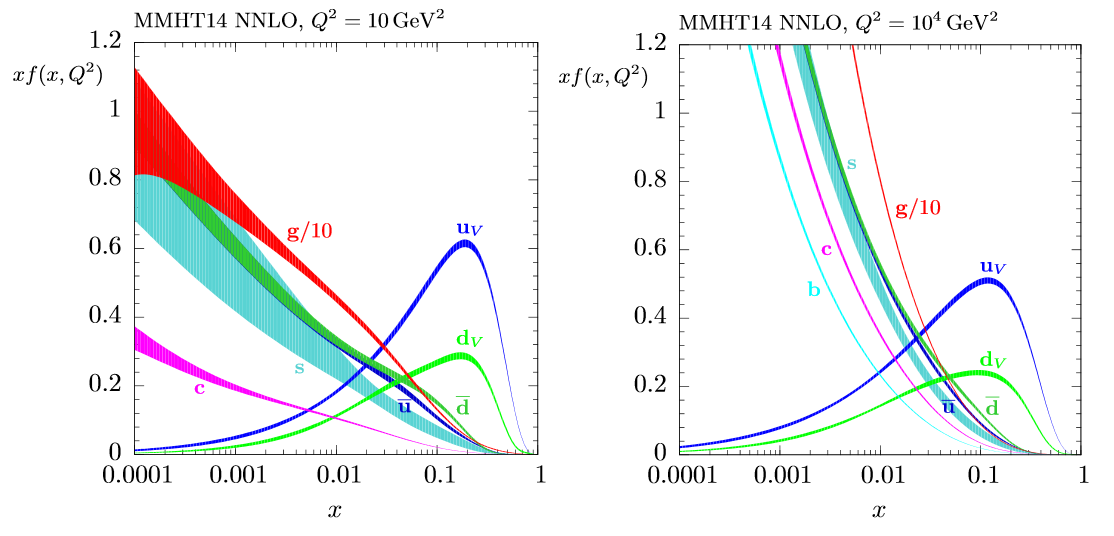
\includegraphics[scale=0.6]{figures/pdf's}
\caption{Parton density function of the proton, taken from $\mathtt{MMHT2014}$ \cite{Harland-Lang:2014zoa} with 68\% confidence level. The parton density function is multiplied by $x$ in order to counteract its peak at $x \to 0$. The parton density function is given at two different factorisaction scales $\mu_F = Q$}\label{fig:pdfs}
\end{center}
\end{figure}
\begin{figure}[!htpb]
\begin{center}
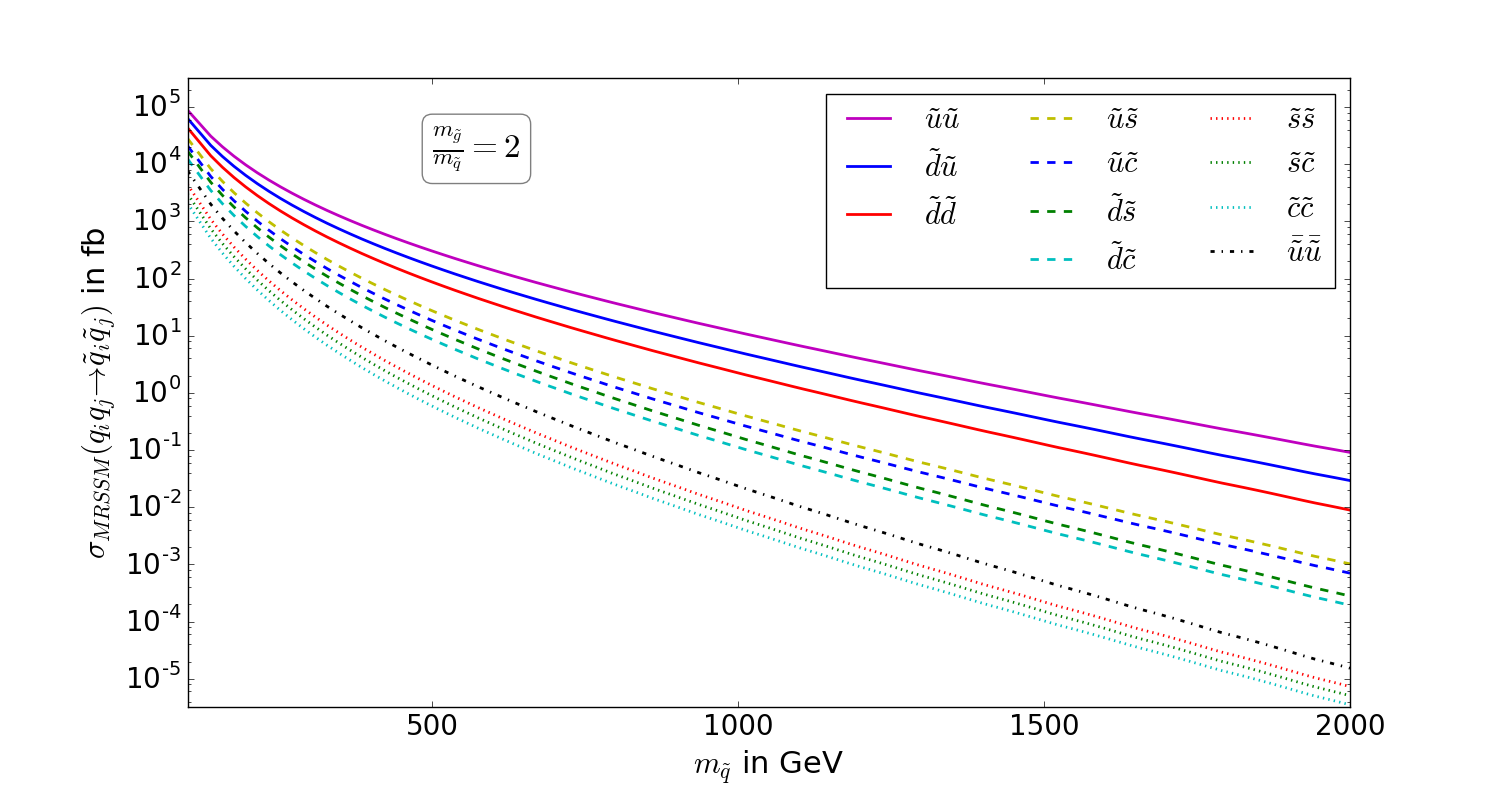
\includegraphics[scale=.45]{figures/MRSSM_q+q_sq+sq_mr=2_seperated}
\caption{Hadronic cross section for squark production in the MRSSM at the LHC at $\sqrt{S} = \unit[13]{GeV}$. The ratio of the gluino and squark mass is fixed to 2. The parton densities used are $\mathtt{MMHT2014}$ LO with $\alpha_s(M_Z) = 0.135$ in the 5-flavor scheme \cite{Harland-Lang:2014zoa}. As renormalization and factorization scale $\mu_R = \mu_F = \frac{m_1 + m_2}{2}$ has been chosen, where $m_i$ are the final state particle masses.} \label{fig:TreeXsection}
\end{center}
\end{figure}\\
They actually depend on an arbitrary energy scale referred to as the factorization scale $\mu_F$. The $\mu_F$ evolution is given within the scope of perturbation theory by coupled integro-differential equations named after Gribov, Lipatov\cite{Gribov:1972ri}, Dokshitzer\cite{Dokshitzer:1977sg}, Altarelli and Parisi\cite{Altarelli:1977zs}: the DGLAP-equations. For further reading on parton density functions and factorization see \cite{dissertori2003quantum} and \cite{Collins:1989gx}. See \cite{Brock:1993sz} for how to determine parton density functions.\\
Fig. \ref{fig:pdfs} shows a parton density function set for the proton. One can see that the partons most probable to carry a high fraction of momentum are the valence quarks. For lower values of $x$, gluons constitute the major component of the proton.\\
Fig.\ref{fig:TreeXsection} shows the hadronic cross section for the production of various squarks in the MRSSM. These can only be produced by their non supersymmetric partner, e.g. two up-squarks can only be produced by two up-quarks. Because the partonic cross section for these processes are the same, cf. eq. \eqref{eq:PartonicEquality}, one can see the influence of the parton density functions quite nicely: The up-squark production is the dominant contribution to squark production. Apart from the solid lines in fig. \ref{fig:TreeXsection} which correspond to the production of first generation squarks, also the cross section of mixed first and second generation (dashed lines) and second generation (dotted lines) squarks is shown. The dashed dotted line shows the cross section of the charged conjugated particles of the dominant channel.\\


\subsection{Results for Squark and Gluino Production at Tree-Level}\label{sec:tree-level_cross_sections}
%REFER TO Kribs, Martin: SNOWMASS WHITEPAPER\\
%REFER TO Vernoica Sanz: How many SUpersymmetries?\\
%\\
This section presents hadronic tree-level (Born) cross sections of squark and gluino production for two colliding protons in both, the MSSM and the MRSSM.\\
Note that in the following all possible production channels are taken into account. This is, for squark and squark-gluino production, also the charged conjugated processes, i.e. $\tilde{q}^\dagger\tilde{q}^\dagger$ and $\tilde{q}^\dagger\tilde{g}\left( \overline{\tilde{g}} \right)$, are included. In addition, squark production counts thoses processes twice which involve flavor unlike quarks, e.g. $ud \to \tilde{u}\tilde{d}$ is counted twice as the $d$-quark may come from either proton. This applies also to squark-antisquark production through a quark-antiquark pair.\\
The calculations have been performed by a $\texttt{C++}$ code which uses a library containing the absolute squared amplitudes for the processes in question. Note that the author has opted for the absolute squared amplitudes and not the partonic cross sections because this allows also for the calculation of partial differential cross sections, for possible future use. To perform the integration over the Mandelstam variable $t$ and $x_1$ and $x_2$, the routine ``Cuhre'' which is part of the \texttt{CUBA} library\cite{Hahn:2004fe} has been used\\
The following paragraph discusses fig. \ref{fig:TreeXsection}, \ref{fig:TreeLevelSigma_0,9_2} and \ref{fig:TreeXsection5}, i.e. the hadronic cross section of all considered processes for three successive mass ratios of gluino and squark: $\frac{m_{\tilde{g}}}{m_{\tilde{q}}} = 0.9,\ 2$ and $5$. Also, the corresponding fraction of final states is shown.
\begin{figure}[!htpb]
\begin{center}
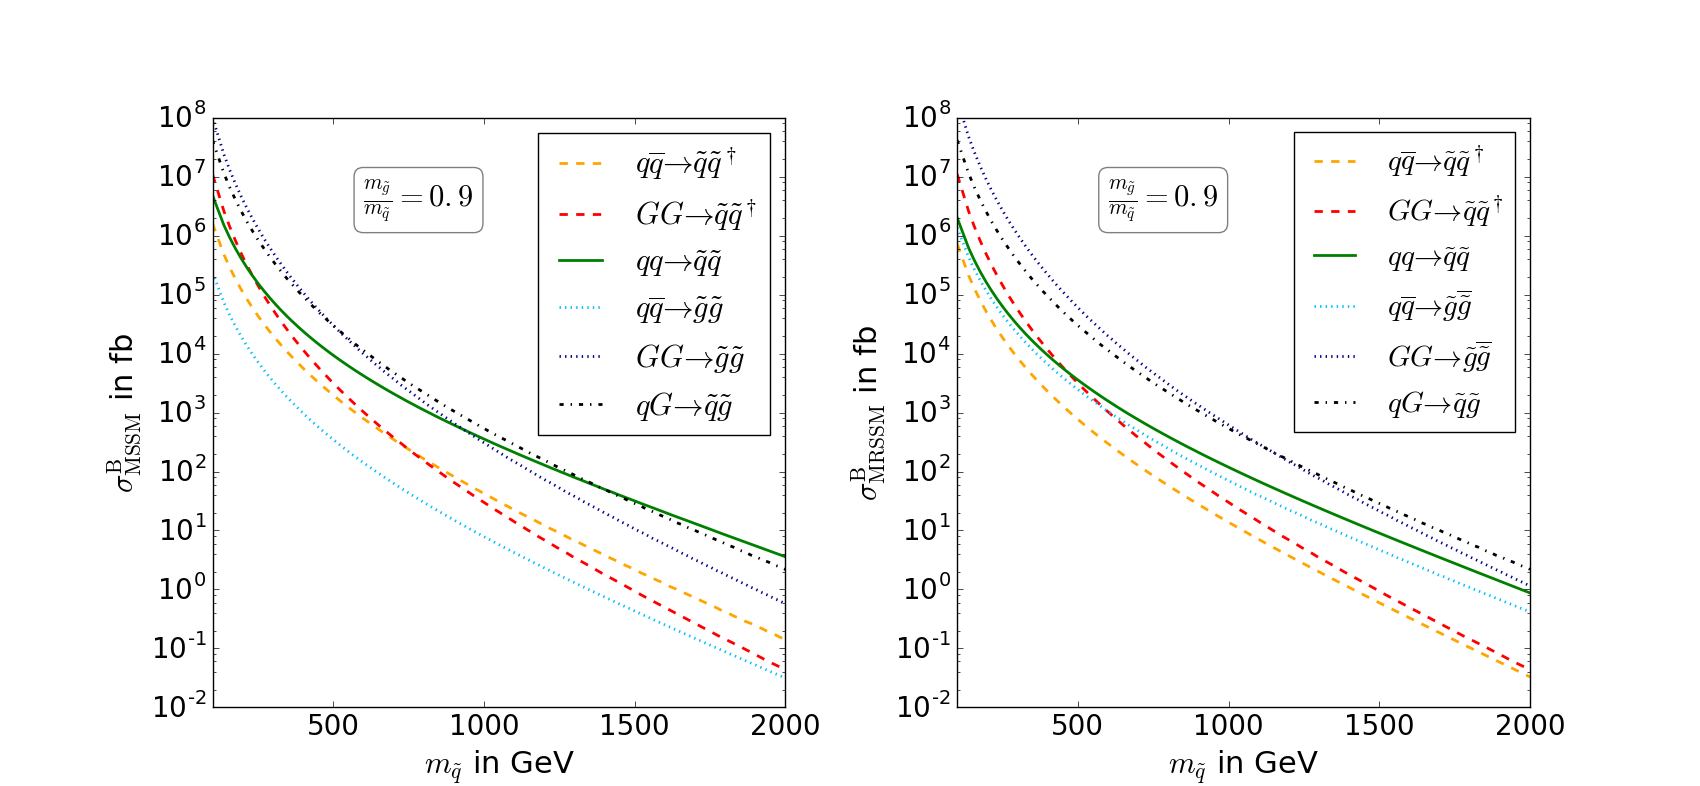
\includegraphics[scale=.4]{figures/mr=0,9_MSSM+MRSSM}
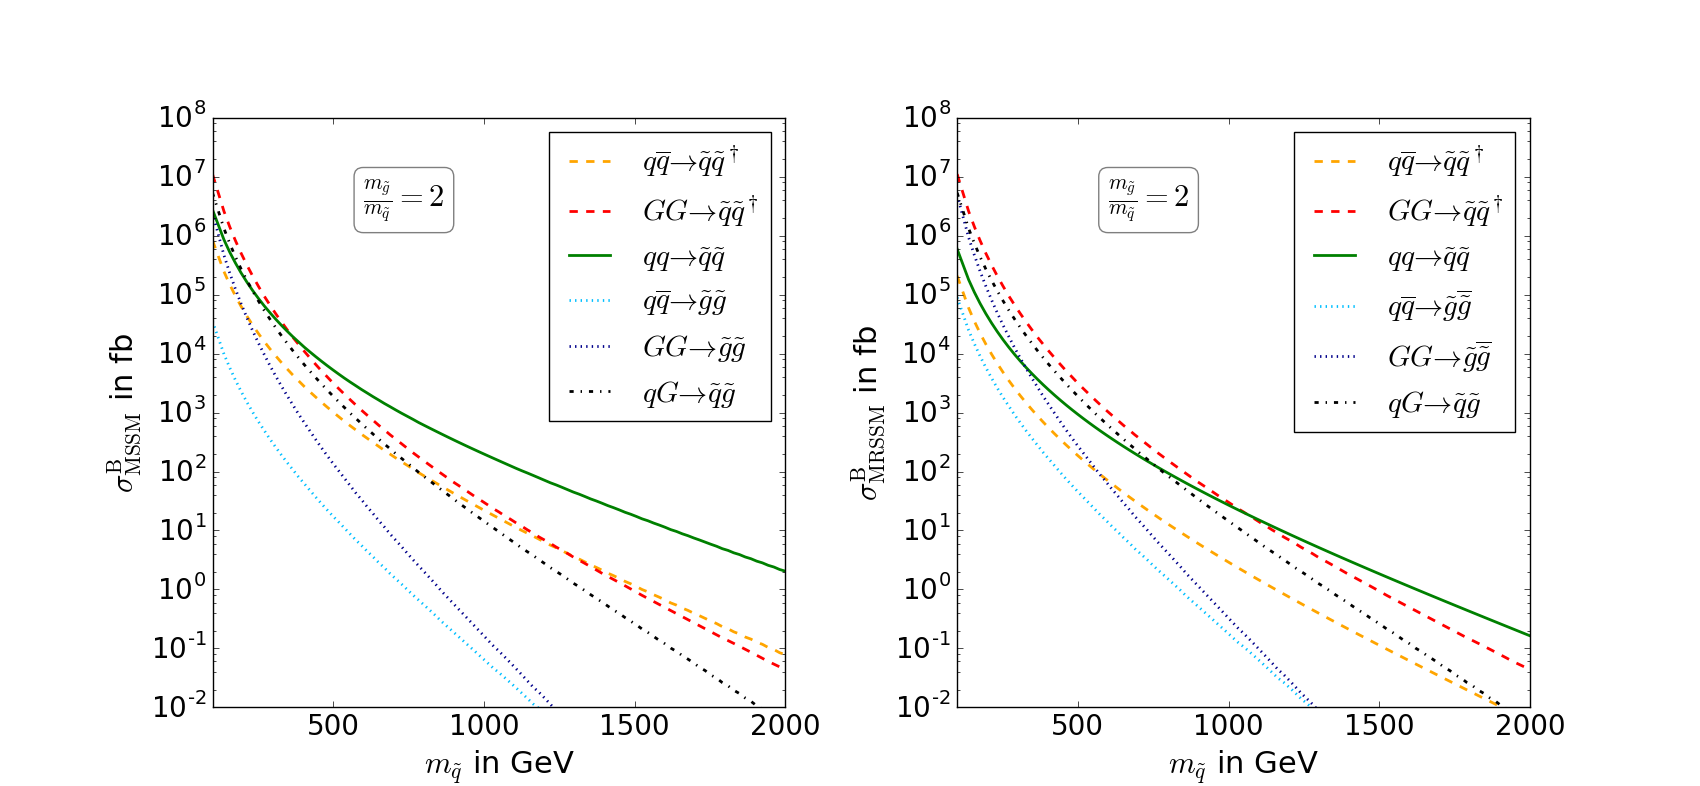
\includegraphics[scale=.4]{figures/mr=2_MSSM+MRSSM}
\caption{Hadronic cross section for squark and gluino production in the MSSM (left-hand side) and MRSSM (right-hand side) at the LHC with $\sqrt{S} = \unit[13]{GeV}$. The ratio of gluino and squark mass is fixed to 0.9 (first row) and 2 (second row). In the final state it has been summed over all squark flavors expect for $t$-squarks. For the channels $qq \to \tilde{q}\tilde{q}$ and $qG \to \tilde{q}\tilde{G}$ also the charge conjugated process is included. The parton densities used are $\mathtt{MMHT2014}$ LO with $\alpha_s(M_Z) = 0.135$ in the 5-flavor scheme \cite{Harland-Lang:2014zoa}. As renormalization and factorization scale $\mu_R = \mu_F = \frac{m_1 + m_2}{2}$ has been chosen, where $m_i$ are the final state particle masses.} \label{fig:TreeXsection}
\end{center}
\end{figure}
\begin{figure}[!htpb]
\begin{center}
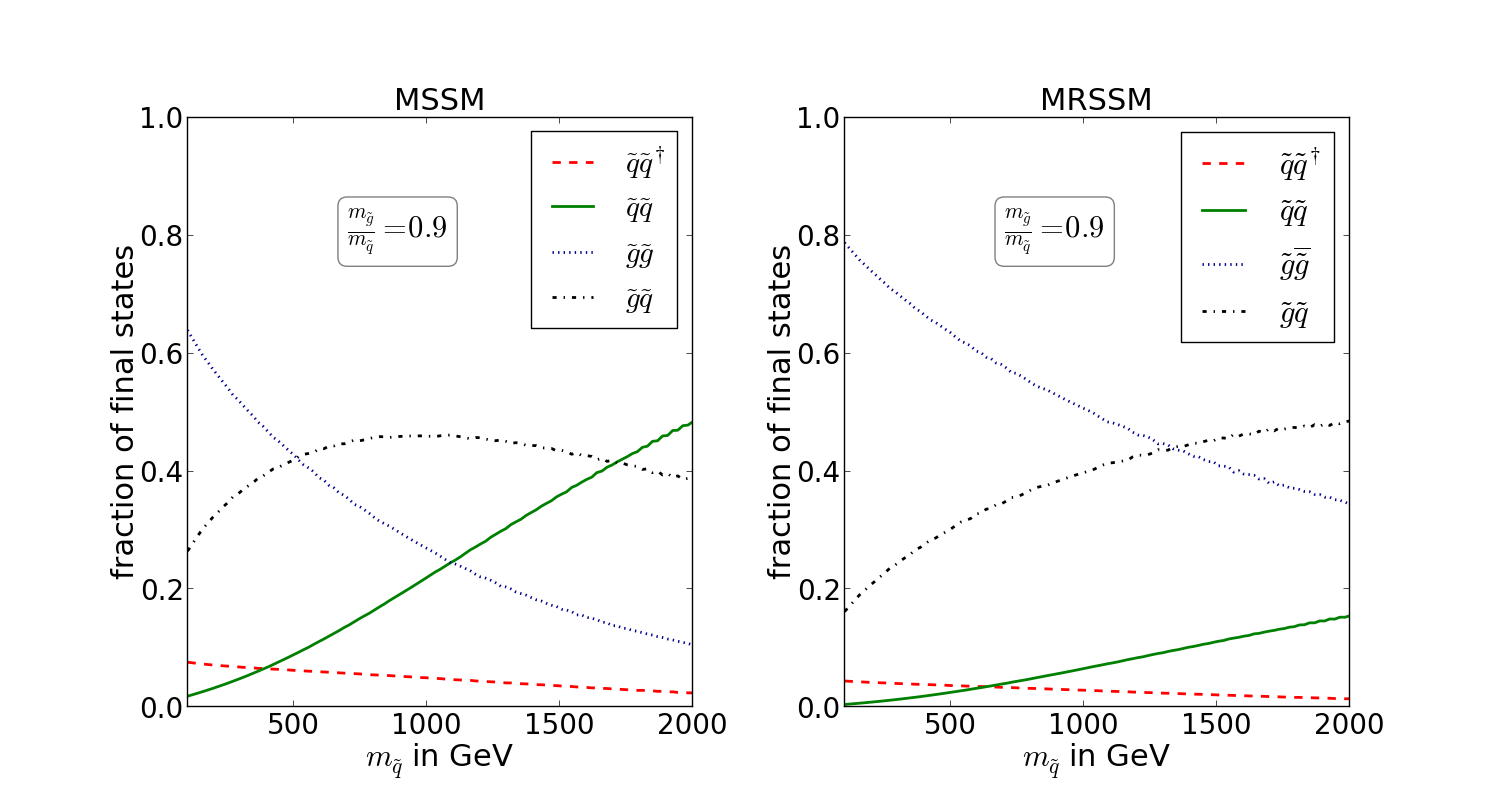
\includegraphics[scale=.45]{figures/rel_weights_mr=0,9_MSSM+MRSSM}
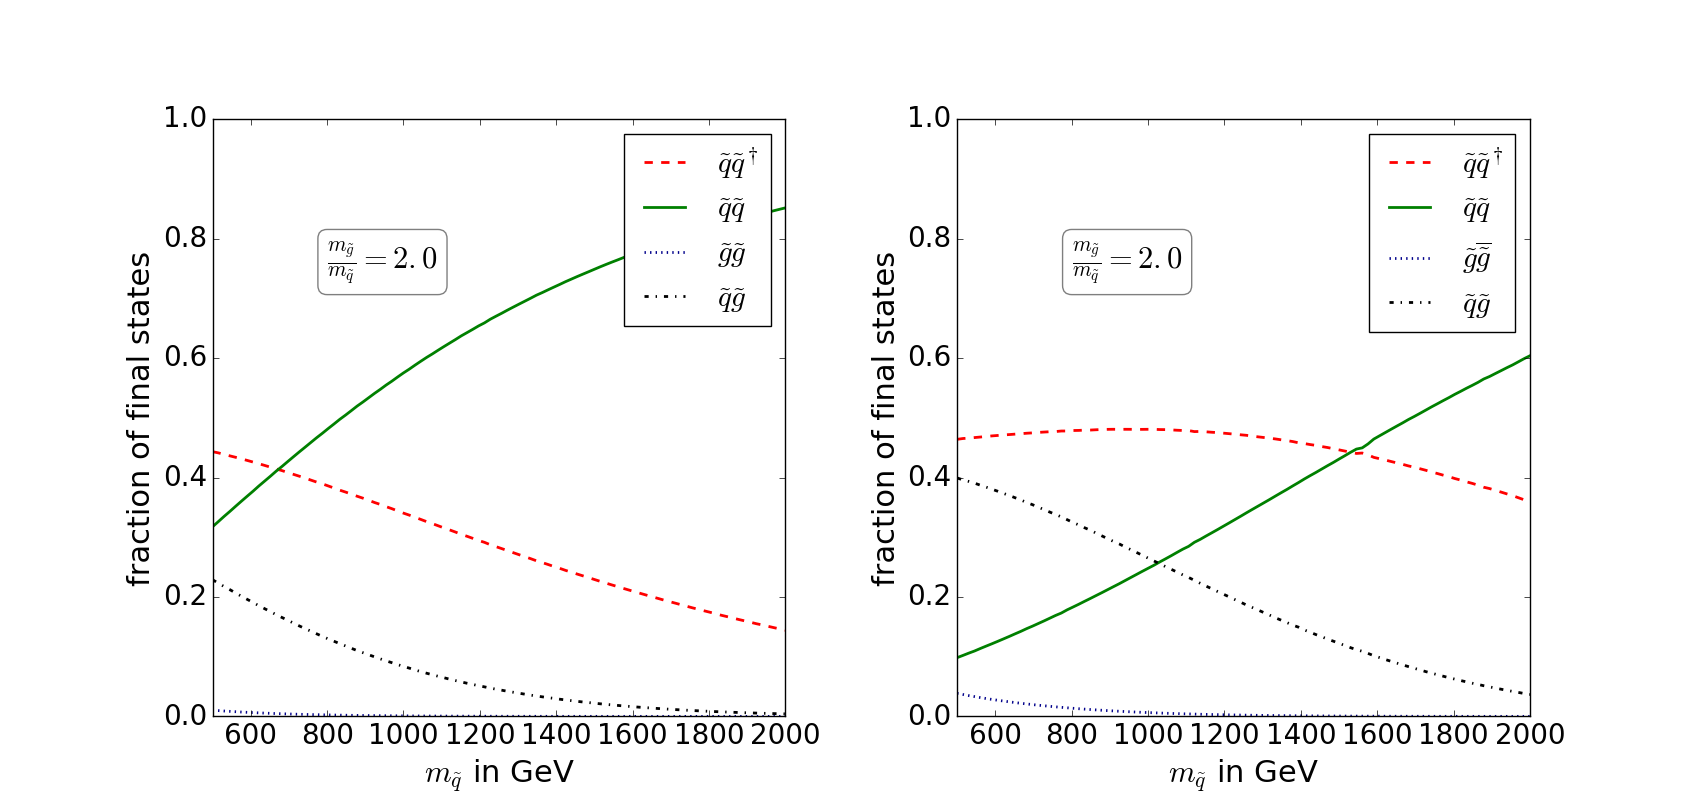
\includegraphics[scale=.45]{figures/rel_weights_mr=2_MSSM+MRSSM}
\caption{Relative contributions of the indicated final states on the total hadronic cross section in the MSSM (left-hand side) and MRSSM (right-hand side) at the LHC with $\sqrt{S} = \unit[13]{GeV}$. The ratio of gluino and squark mass is fixed to 0.9 (first row) and 2 (second row). In the final state it has been summed over all squark flavors expect for $t$-quarks. For the channels $qq \to \tilde{q}\tilde{q}$ and $qG \to \tilde{q}\tilde{G}$ also the charge conjugated process is included. The parton densities and the renormalization and factorization scale are chosen as in fig. \ref{fig:TreeXsection}.}\label{fig:TreeLevelSigma_0,9_2}
\end{center}
\end{figure}

For the small mass ratio $\frac{m_{\tilde{g}}}{m_{\tilde{q}}} = 0.9$ and small squark masses, the dominant contribution comes from gluino (antigluino) production. This is even more dominant in the MRSSM which can be explained by the above mentioned factor of two difference in the $GG \to \tilde{g}\tilde{g}(\overline{\tilde{g}})$ channel which comes from the distinguishable gluino and antigluino in the MRSSM. Furthermore there is the above mentioned destructive interference term in the $q\overline{q} \to \tilde{g}\tilde{g}(\overline{\tilde{g}})$ channel which makes the cross section for this process in the MRSSM dominant over the one in the MSSM.\\
For a growing squark mass the previously subdominant gluino-squark production takes over and becomes dominant. A salient difference between the MSSM and the MRSSM is that squark production is strongly suppressed in the MRSSM. While in the MSSM it becomes dominant above about $\unit[1400]{GeV}$ it is subsubdominant for the whole displayed squark mass in the MRSSM. This suppression has also already been explained above.\\
Turning from $\frac{m_{\tilde{g}}}{m_{\tilde{q}}} = 0.9$ to $\frac{m_{\tilde{g}}}{m_{\tilde{q}}} = 2$ suppresses quite strongly the production of gluinos in all pertaining channels. For the MSSM one finds above $\unit[500]{GeV}$ a growing dominance of squark production. The same happens in the MRSSM but for a significantly higher squark mass of about $\unit[1200]{GeV}$. This suppression of squark production in the MRSSM increases with a growing gluino masses which can be seen when going from $\frac{m_{\tilde{g}}}{m_{\tilde{q}}} = 0.9$ to  $\frac{m_{\tilde{g}}}{m_{\tilde{q}}} = 2$ or even $\frac{m_{\tilde{g}}}{m_{\tilde{q}}} = 5$ depicted in fig. \ref{fig:TreeXsection5}. This reflects the gluino mass dependence explained in detail in section \ref{sec:PartProcesses}. See also \ref{fig:TreeXsection_fixed_m} for a visualization of this behavior.\\
Note also, that for sufficiently large squark masses squark production becomes the dominant process, see fig. \ref{fig:TreeXsection} and \ref{fig:TreeLevelSigma_0,9_2}. This is because the production of heavy particles requires large longitudinal momenta of the colliding partons, i.e. large $x$. Looking at the parton density functions in fig. \ref{fig:pdfs} one sees that within the proton the partons most likely to carry large momentum are quarks. So looking at large $x$ the proton basically consists of quarks and because the only process involving only quarks in the initial state is squark production, this channel dominates for high masses.\\
The total cross section in the MRSSM is increasingly smaller than in the MSSM in particular from about $\unit[500]{GeV}$ onwards. The is because for masses below that the $GG \to \tilde{q}\tilde{q}^\dagger$ channel, which is the same for both models, is the dominant one.\\
When raising the gluino squark mass ratio further to $\frac{m_{\tilde{g}}}{m_{\tilde{q}}} = 5$ the above described tendency continues. This is, all processes including a gluino get even more negligible and squark production gets further suppressed. While in the MSSM it becomes dominant over $GG \to \tilde{q}\tilde{q}^\dagger$ at $m_{\tilde{q}} \approx \unit[800]{GeV}$, it is subdominant in the MRSSM within the whole displayed mass range, even though it does not fall that steeply as the dominant channel.\\

\begin{figure}[!htpb]
\begin{center}
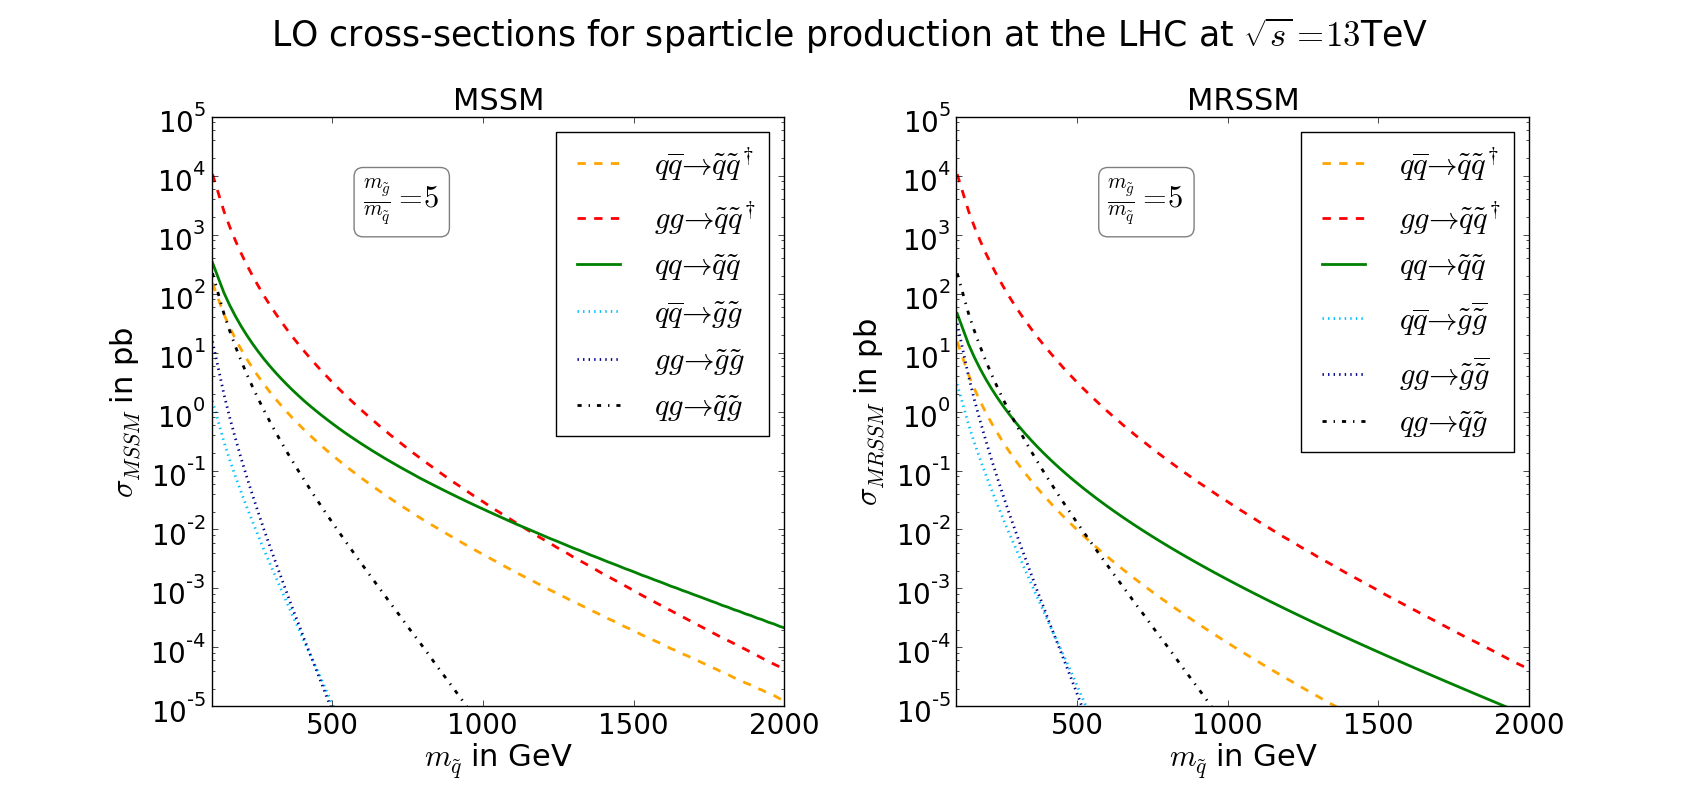
\includegraphics[scale=.4]{figures/mr=5_MSSM+MRSSM}
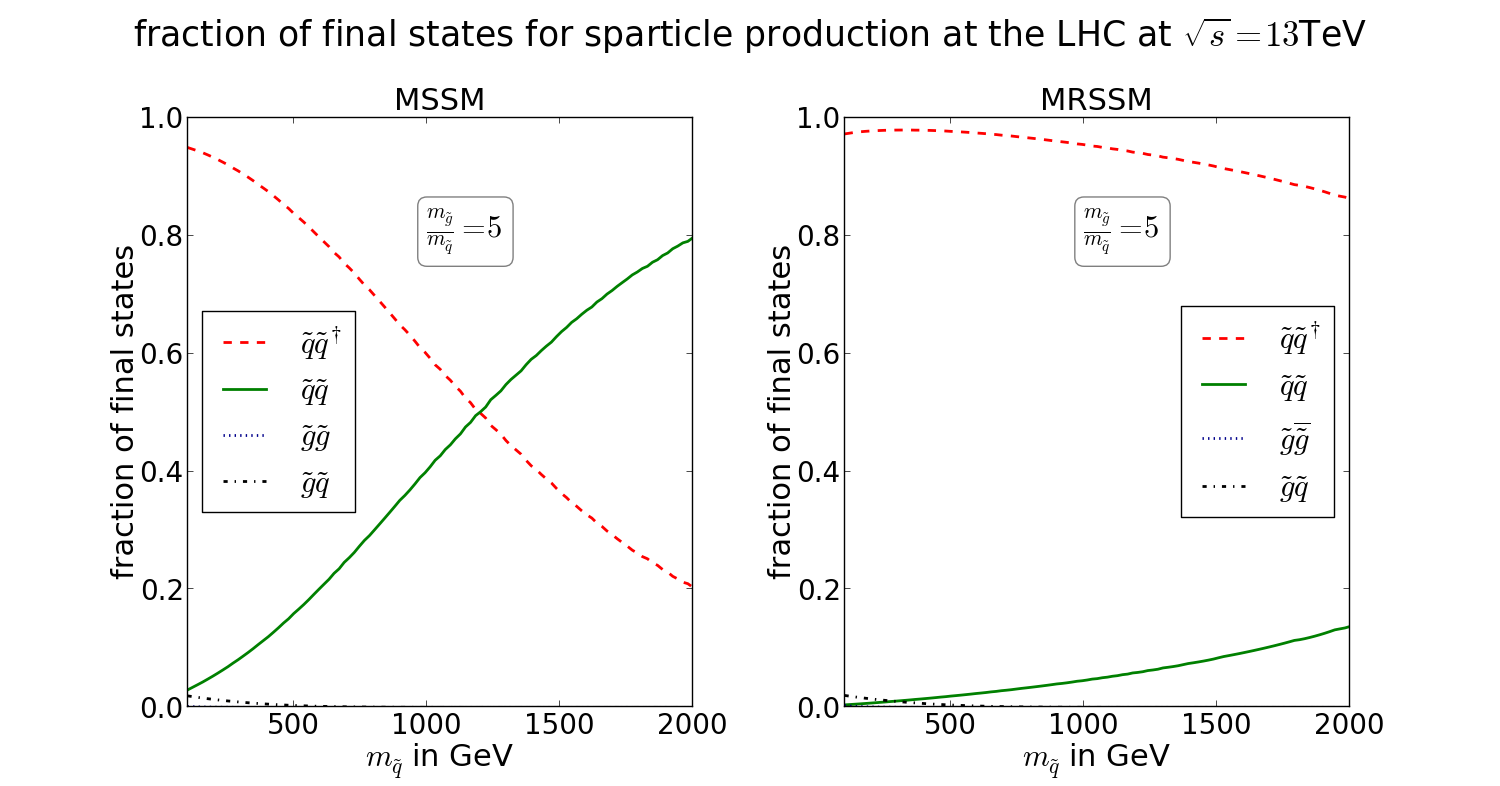
\includegraphics[scale=.45]{figures/rel_weights_mr=5_MSSM+MRSSM}
\caption{Hadronic cross section for squark and gluino production (in the first row) and relative contributions of the indicated final states on the total hadronic cross section (in the second row) in the MSSM (left-hand side) and MRSSM (right-hand side) at the LHC which $\sqrt{S} = \unit[13]{GeV}$. The ratio of gluino and squark mass is fixed to 5. In the final state it has been summed over all squark flavors expect for staus. For the channels $qq \to \tilde{q}\tilde{q}$ and $qG \to \tilde{q}\tilde{G}$ also the charge conjugated process is included. The parton density functions and the renormalization and factorization scale are chosen as in fig. \ref{fig:TreeXsection}.}\label{fig:TreeXsection5}
\end{center}
\end{figure}
\newpage
The contour plots in fig. \ref{fig:ContourTree} underline the already announced difference between squark production in the MRSSM and the MSSM. While the cross sections for small gluino masses resemble each other closely, the cross section in the MRSSM gets increasingly suppressed with increasing gluino mass. 
\begin{figure}[!htpb]
\begin{center}
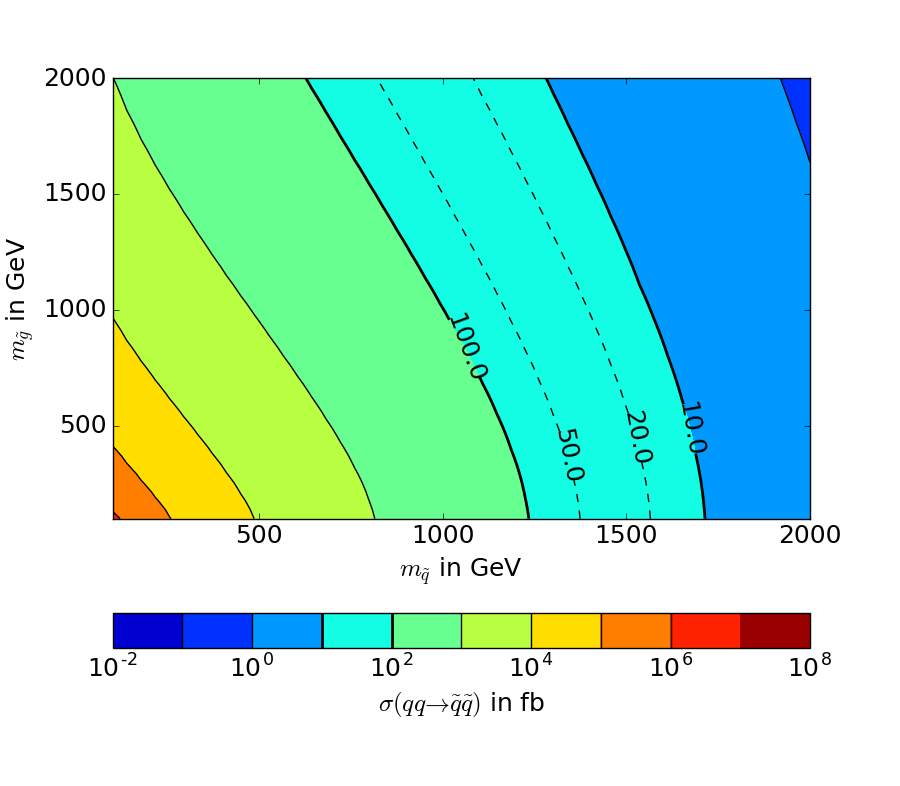
\includegraphics[scale=.55]{figures/contour_MRSSM_squarks}
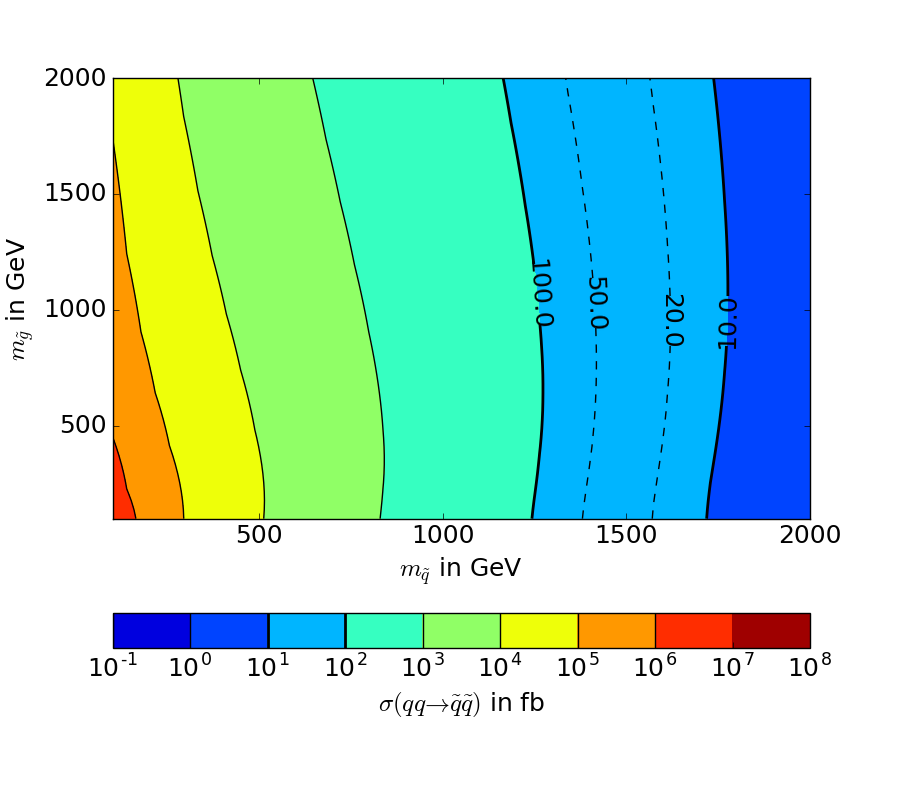
\includegraphics[scale=.55]{figures/contour_MSSM_squarks}
\caption{The squark production cross section including five flavors (also including $\tilde{q}^\dagger\tilde{q}^{\prime\dagger}$) in the MRSSM (top) and MSSM (bottom) at the LHC which $\sqrt{S} = \unit[13]{GeV}$. The parton density functions and the renormalization and factorization scale are chosen as in fig. \ref{fig:TreeXsection}.}\label{fig:ContourTree}
\end{center}
\end{figure}

\begin{figure}[!htpb]
\begin{center}
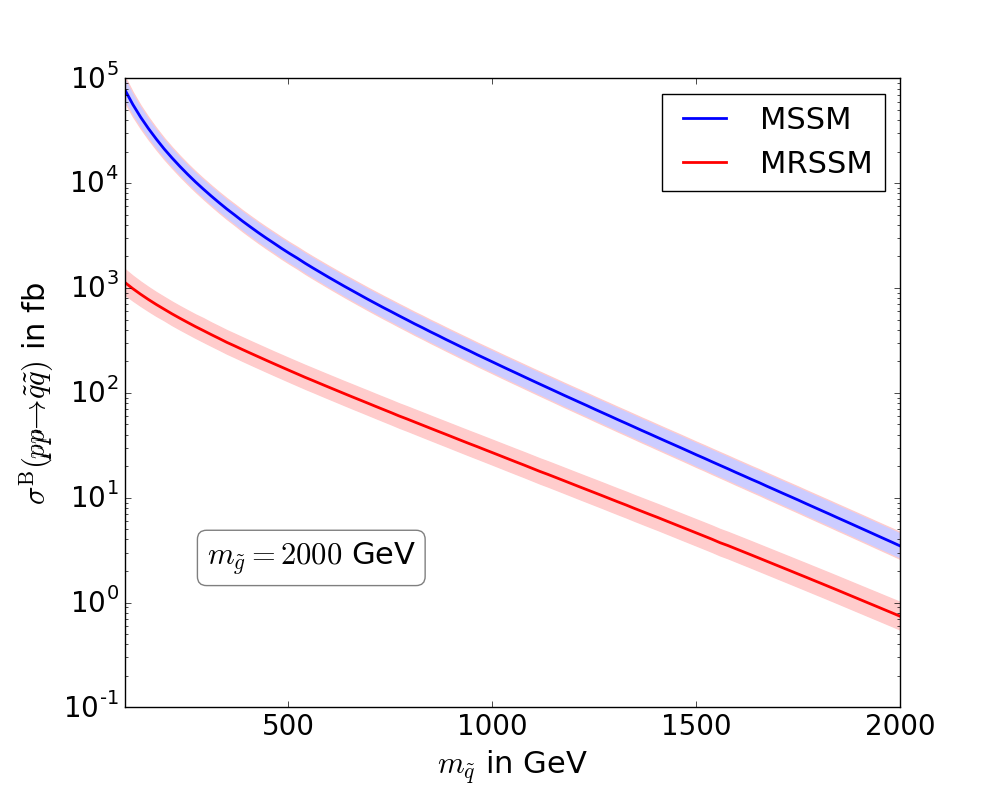
\includegraphics[scale=.5]{figures/MSSM+MRSSM_msg=2000}
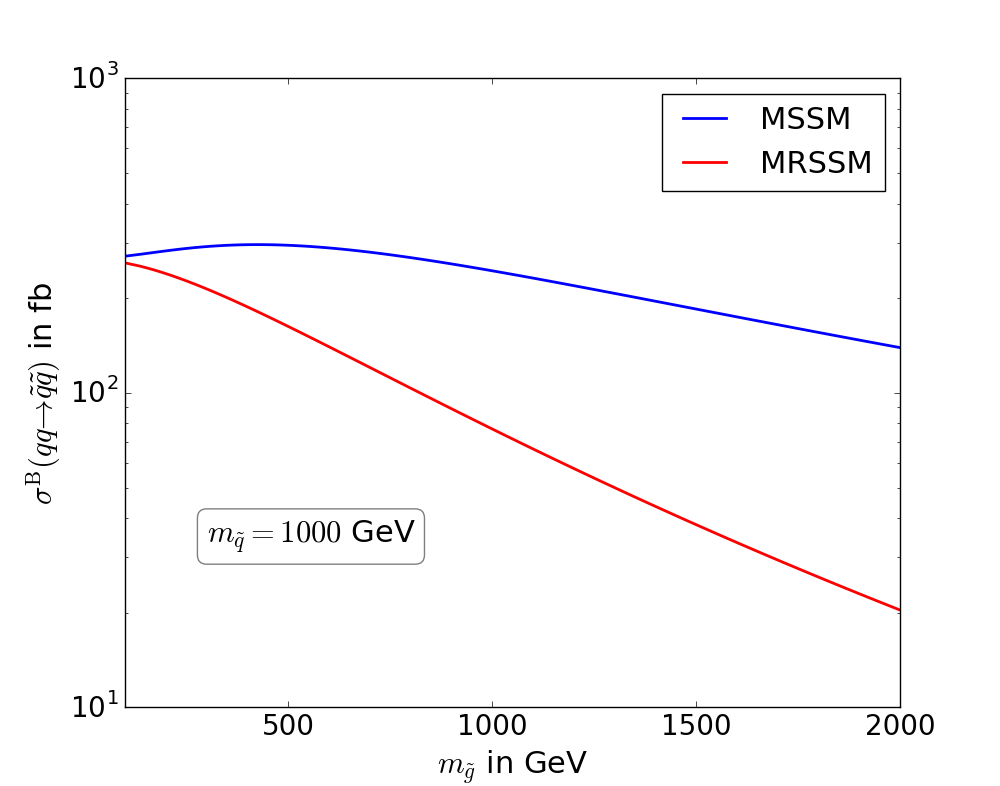
\includegraphics[scale=.5]{figures/MSSM+MRSSM_msq=1000}
\caption{Comparison of squark production cross section including five flavors (also including $\tilde{q}^\dagger\tilde{q}^{\prime\dagger}$) in the MSSM and MRSSM at the LHC which $\sqrt{S} = \unit[13]{GeV}$ for fixed gluino mass (top) and fixed squark mass (bottom). The parton density functions and the renormalization and factorization scale are chosen as in fig. \ref{fig:TreeXsection}.}\label{fig:TreeXsection_fixed_m}
\end{center}
\end{figure}

Fig.\ref{fig:TreeXsection_fixed_m} shows the Born cross section of squark production including all possible flavors for a fixed mass of the gluino $m_{\tilde{g}} = \unit[2000]{GeV}$ (top) and the squark $m_{\tilde{q}} = \unit[1000]{GeV}$ (bottom). The figure includes errors of the calculation which come from the parton density functions and the renormalization and factorization scale.\\
The 68\% uncertainty from the central value pdf-set is obtained by performing the calculation with all eigenvector sets of the central value and taking the minimum and maximum at each point as deviations from the calculation with the central set.\\
The uncertainty from the renormalization scale $\mu_R$ and the factorization scale $\mu_F$ is obtained by varying both parameters with a factor of $\frac{1}{2}$ and two. For each parameter combination the cross section has been calculated. The uncertainty originating from the scale has then been determined by taking the minimum and maximum of these nine numbers for each point.\\
The total uncertainty is then obtained by Gauß's propagation of uncertainties:
\begin{align}
\Delta \sigma = \sqrt{(\Delta \sigma_{\mathrm{pdf}})^2 + (\Delta \sigma_{\mathrm{scale}})^2}.
\end{align}
The uncertainty coming from the scale variation has been found much greater than the one from the parton density functions. The uncertainty from the phase space integration is negligible, i.e. $\Delta \sigma_{\mathrm{int}} < 1\text{\textperthousand}$.
\newpage

\begin{table}[H]
\begin{center}
\begin{tabular}{c?c|c|c}
\backslashbox{$m_{\tilde{g}}$}{$m_{\tilde{q}}$} & $\unit[500]{GeV}$ & $\unit[1000]{GeV}$ & $\unit[1500]{GeV}$\\
\hlinewd{2pt}
& & & \\
$\unit[1000]{GeV}$ & $\unit[934.9]{fb}\ _{- 27.2\%\ignore{735}- 2.1\% \ignore{915}}^{+ 30.0\% \ignore{1213}+ 1.2\% \ignore{946}}$ & $\unit[102.1]{fb}\ _{- 29.2\% \ignore{79.0}- 2.1\%\ignore{100}}^{+ 31.2\% \ignore{134}+ 1.9\% \ignore{104}}$ & $\unit[13.12]{fb}\ _{- 31.6\% \ignore{9.97}- 1.7\% \ignore{12.9}}^{+ 34.1\% \ignore{17.6}+ 2.1\% \ignore{13.4}}$\\
& & & \\
$\unit[1500]{GeV}$ & $\unit[360.9]{fb}\ _{- 30.0\% \ignore{282}- 2.2\% \ignore{353}}^{+ 30.5\% \ignore{471}+ 1.1\% \ignore{365}}$ & $\unit[50.52]{fb}\ _{- 29.5\% \ignore{39.0}- 1.9\% \ignore{49.6}}^{+ 32.4\% \ignore{66.9}+ 1.7\% \ignore{51.4}}$ & $\unit[7.712]{fb}\ _{- 31.8\% \ignore{5.85}- 2.8\% \ignore{7.5}}^{+ 34.9\% \ignore{10.4}+ 2.4\% \ignore{7.9}}$\\
& & & \\
$\unit[2000]{GeV}$ & $\unit[165.5]{fb}\ _{- 28.2\% \ignore{129}- 2.1\% \ignore{162}}^{+ 30.5\% \ignore{216}+ 0.9\% \ignore{167}}$ & $\unit[26.97]{fb}\ _{- 29.8\%\ignore{20.8}- 2.1\% \ignore{26.4}}^{+ 32.6\%\ignore{35.8} + 1.5\% \ignore{27.4}}$ & $\unit[4.625]{fb}\ _{- 31.8\% \ignore{3.51}- 1.6\% \ignore{4.55}}^{+ 34.5\% \ignore{6.22}+ 1.8\% \ignore{4.71}}$\\
\end{tabular}
\caption{Squark production cross section at tree-level (including five flavors and also the production of antisquarks) in the MRSSM for various squark and gluino masses. The uncertainty of the numerical integration is lower than one permille. The first relative uncertainty comes from the variation of $\mu_R$ and $\mu_F$ as described in the text. The second uncertainty corresponds to the parton density function uncertainty.}\label{tab:squarkMRSSM}
\end{center}
\end{table}
%\vspace{1cm}
\begin{table}[H]
\begin{center}
\begin{tabular}{c?c|c|c}
\backslashbox{$m_{\tilde{g}}$}{$m_{\tilde{q}}$} & $\unit[500]{GeV}$ & $\unit[1000]{GeV}$ & $\unit[1500]{GeV}$\\
\hlinewd{2pt}
& & & \\
$\unit[1000]{GeV}$ & $\unit[5257]{fb}\ _{- 24.6\% \ignore{4196}- 1.2\% \ignore{5163}}^{+ 28.4\% \ignore{6714}+ 1.8\% \ignore{5319}}$ 
& $\unit[340.4]{fb}\ _{- 28.4\% \ignore{265}- 1.9\% \ignore{334}}^{+ 31.0\% \ignore{446} + 1.6\% \ignore{346}}$ 
& $\unit[33.97]{fb}\ _{\- 30.6\% \ignore{26.0}- 1.2\%\ignore{33.5}}^{+ 33.6\% \ignore{45.4}+ 2.3\%\ignore{34.7}}$\\
& & & \\
$\unit[1500]{GeV}$ & $\unit[3263]{fb}\ _{- 25.4\% \ignore{2602}- 1.8\%\ignore{3205}}^{+ 27.9\%\ignore{4172}+ 1.2\%\ignore{3301}}$ 
& $\unit[260.7]{fb}\ _{- 28.4\%\ignore{203}- 2.2\%\ignore{255}}^{+ 30.8\% \ignore{341}+ 1.3\% \ignore{264}}$ 
& $\unit[30.46]{fb}\ _{- 30.7\%\ignore{23.3} - 1.9\%\ignore{29.9}}^{+  33.2\% \ignore{40.6} + 1.8\% \ignore{31.0}}$\\
& & & \\
$\unit[2000]{GeV}$ & $\unit[2179]{fb}\ _{- 25.6\% \ignore{1735}- 1.9\%\ignore{2139}}^{+ 27.9\% \ignore{2788}+ 1.1\%\ignore{2204}}$ 
& $\unit[198.1]{fb}\ ^{+ 30.7\%\ignore{259} + 1.5\%\ignore{201}}_{- 28.6\% \ignore{154}- 2.1\%\ignore{194}}$ 
& $\unit[25.75]{fb}\ ^{+ 33.2\%\ignore{34.3}+ 1.5\%\ignore{26.2}}_{- 30.7\% \ignore{19.7}- 2.0\%\ignore{25.3}}$\\
\end{tabular}
\caption{Same content as in \ref{tab:squarkMRSSM} but for the MSSM.}
\end{center}
\end{table}

As a summary of the comparison between MSSM and MRSSM, one can say, that the gluino production is enhanced in the MRSSM due to distinguishable gluino and antigluino. In order to meet missing experimental evidence for supersymmerty, this suggests that gluinos might be heavier than squarks in the MRSSM. Focusing on $\frac{m_{\tilde{g}}}{m_{\tilde{q}}} \geq 2$ the most significant change between the considered models is the growing suppression of squark production for an increasing gluino mass. This is why this channel is going to be investigated at next-to-leading order within this thesis. The ensuing sections provide the prerequisites for this calculation.